% !TEX program = pdflatex
% !BIB program = bibtex
\documentclass[a4paper,10pt,twoside]{article}

\setlength{\parskip}{2mm}


\usepackage[utf8]{inputenc}
\usepackage{amsfonts}
\usepackage{amsmath}
\usepackage{mathpazo}
\usepackage{multicol}
\usepackage{amssymb}
\usepackage{amsthm}
% \usepackage{setspace}
\usepackage{fancybox}
\usepackage[spanish]{babel}
\usepackage[T1]{fontenc}
%\usepackage[pdftex]{graphicx} %Utilizarlo sólo si voy a compilar con pdftex y tengo imágenes pixeladas (no vectoriales) con las gráficas.
\usepackage{cancel}
\usepackage{fancyhdr}
\usepackage{eurosym}
\usepackage[dvips]{graphicx}%Utilizarlo para  cargar archivo de extensión *.eps (gráficos vectoriales)en el documento
\DeclareGraphicsExtensions{.png,.pdf,.jpg}
\usepackage{pstricks-add}%Utilizarlo para cargar código ps-tricks de geogebra por ejemplo (no usar con \usepackage[pdftex]{graphicx})
\usepackage[colorlinks=true,linkcolor=blue]{hyperref}
\usepackage{hyperref}
\hypersetup{
    colorlinks,%
    citecolor=black,%
    filecolor=black,%
    linkcolor=black,%
    urlcolor=black
}
\usepackage{wrapfig}
\usepackage{textcomp}
\usepackage{nonfloat}%para poder poner notas al pie en los pies de Figuras o de Tablas
                     %\begin{minipage}{\textwidth}
                     %   \centering
                     %   \begin{tabular}{|c|}
                     %      \hline  Tabular stuff here \\ \hline
                     %   \end{tabular}
                     %   \tabcaption[Text of the caption (second example)]{Text of the caption (second example)\footnotemark}
                     % \end{minipage}
                     % \\[\intextsep]
                     %\footnotetext{Text of the footnote (second example)}
\usepackage{colortbl}%Para colores en tablas
\usepackage{verbatim} %Para utilizar comentarios comentarios
\usepackage{fixltx2e}% superíndices y subindices (\textsubscript{} y \textsuperscript{}) en modo texto

%Nueva geometría de la página, con respecto a la de por defecto
\usepackage[text={14.7cm,22.6cm},centering]{geometry}
\addtolength{\headsep}{-0.35cm}
\addtolength{\footskip}{-0.3cm}
\addtolength{\voffset}{0.6cm}%{-0.65cm}
\addtolength{\hoffset}{-0.05cm}%{-0.65cm}

% Tikz graphics
\usepackage{tikz}
\usetikzlibrary{positioning}
% Tablas bonitas
\usepackage{booktabs}
% Tablas apaisadas
\usepackage{pdflscape}
% Múltiples líneas en tablas
\usepackage{multirow}
% Listas
\usepackage[inline]{enumitem}

% Definiciones y ejemplos
\theoremstyle{definition}
\newtheorem{definition}{Definición}
\newtheorem{example}{Ejemplo} 

% Colores
\definecolor{color1}{RGB}{5,161,230} % Azul
\definecolor{color2}{RGB}{230,37,52} % Rojo

%%%%% Para los encabezados y pies de Página
\pagestyle{fancy}
\lhead[\scriptsize{\textit{\href{mailto:asalber@ceu.es}{Alfredo Sánchez Alberca}}}]{\scriptsize{\textit{Taxonomía de colecciones y funciones de similitud}}} % a completar por equipo editorial
\chead{}
\rhead[\scriptsize{\textit{Taxonomía de colecciones y funciones de similitud}}]{\scriptsize{\textit{\href{mailto:asalber@ceu.es}{Alfredo Sánchez Alberca}}}} % a completar por equipo editorial
\lfoot[\thepage \ \  |  \ \scriptsize{\textit{5\textsuperscript{as} Jornadas ``Matemáticas Everywhere''}}]{\scriptsize{\textit{18, 19 y 20 de junio de 2018, Castro Urdiales}}}% a completar por equipo editorial
\cfoot{}
\rfoot[\scriptsize{\textit{18, 19 y 20 de junio de 2018, Castro Urdiales}}]{\scriptsize{\textit{5\textsuperscript{as} Jornadas ``Matemáticas Everywhere''}}\ \ \ \normalsize{|} \   \thepage}
%%%%% Fin de encabezados y pies de página

%%%%% Genera los pies de Figuras y Tablas en itálicas y a tamaño footnote
\usepackage[font={footnotesize,it}, format=plain, labelformat=simple, labelsep=period, center]{caption}
\renewcommand\thefigure{\arabic{figure}} % Genera numeración X
\renewcommand\thetable{\arabic{table}} % Genera numeración X

\setcounter{page}{1}%para comenzar la numeración de las páginas en documentos. Dejar 1 por defecto.



\begin{document}
%Cambiar Palabra Cuadros por Tablas
\renewcommand{\tablename}{Tabla} 

\title{\vspace{-8mm}5\textsuperscript{as} Jornadas ``Matemáticas Everywhere''\\\vspace{4mm}
Una nueva taxonomía de colecciones y de funciones de similitud para su comparación\\\vspace{4mm}
A new taxonomy of collections and similarity functions for comparing them\vspace{-3mm}}  %Para poner el título del artículo
\author{\href{mailto:asalber@ceu.es}{Alfredo Sánchez Alberca}\\ \vspace{2mm} %pone el nombre del autor
\scriptsize Organizan:\\
\small \href{http://www.caminos.upm.es/matematicas/jornadas2014/}{\includegraphics[height=12.5mm]{logos_castro_2014.eps}}\\
\scriptsize Centro Internacional de Encuentros Matemáticos\vspace{-2mm}\\ 
\scriptsize Castro Urdiales, España} %xxx-yyy son las páginas inicial y final respectivamente
\date{18, 19 y 20 de junio de 2018}
%indispensable que al compilarlo se tenga en el mismo directorio raíz el archivo logomirinconbyn.eps que facilito en la descarga.
\maketitle

\begin{abstract}
Las colecciones de objetos, entendidas como agrupaciones de objetos con entidad propia, están presentes en todos los ámbitos de nuestro mundo. 
Aunque no existe aún una definición matemática formal de colección, las colecciones se usan en muchas aplicaciones científicas, y especialmente en ciencias de la computación, donde se utilizan distintas estructuras de datos y con distintas propiedades para representarlas.

En este artículo se presenta una nueva clasificación taxonómica de los tipos de colecciones más comunes organizada de acuerdo a cuatro propiedades estructurales: homogeneidad, unicidad, orden y cardinalidad. 
Sobre la base de esta taxonomía se presenta un catálogo de funciones de similitud para comparar los distintos tipos de colecciones. 
Este catálogo resulta útil para identificar las funciones de similitud más apropiadas para comparar dos colecciones dadas y aplicarlas automáticamente. \\
\newline
\noindent\textbf{Palabras Clave:} Colección, Similitud, Disimilitud, Distancia, Taxonomía. 
\newline
\begin{center}
 \textbf{Abstract}
\end{center}

\vspace{1.2mm}
Collections of objects, understood as groups of objects with its own right, are present all over the world.
Despite of the fact that there is no formal mathematical definition of collection, collections are used in many applications of Science.
In Computer Sciences, in particular, collections are represented by different data structures with different properties.

This paper presents a new taxonomic classification of the most common types of collections organized according to four estructural properties: homogeneity, unity, order and cardinality. 
Based on this taxonomy we also present a catalog of similarity functions for comparing the different types of collections.
This catalog is helpful to identify the most suitable similarity functions to compare two given collections and apply them automatically.\\
\newline
\noindent\textbf{Keywords:} Collection, Similarity, Dissimilarity, Distance, Taxonomy.

\end{abstract}

\section{Introducción}
Las colecciones de objetos, entendidas como agrupaciones o agregaciones de elementos u objetos de diversa índole, están presentes en prácticamente todos los ámbitos de nuestro mundo: los libros de una biblioteca, los alumnos de un curso, los productos de una tienda, los eventos de una agenda, los genes de un individuo, los elementos químicos que componen una sustancia, los trenes que hacen un determinado recorrido, los pixels de una foto y las fotos de un álbum, los jugadores de un equipo y los equipos de una liga, el ranking en una competición, los cartas que llegan a una oficina
de correos, los platos de un menú, los menús de un restaurante y los restaurantes de una ciudad, etc.
Cualquier aplicación o sistema inteligente que pretenda abordar un problema en el que aparezcan colecciones deberá disponer de un sistema de modelado y representación de estas.
Así, en el ámbito de las ciencias de la computación, las colecciones de objetos están presentes de manera explícita en prácticamente todos los sistemas de información, desde los simples arrays en los lenguajes de programación, hasta los registros en las bases de datos, pasando por las listas de procesos, las colas de impresión, o estructuras de datos como los conjuntos, las bolsas, etc., y en última instancia, todo se reduce a colecciones de bits. 

Sin embargo, no hay una correspondencia clara entre las colecciones del mundo real y el modelo o estructura de datos más apropiada para representarla, porque esto depende del nivel de abstracción que se haga y de las primitivas de representación de que disponga un determinado sistema. 
A veces se utiliza una misma estructura de datos para representar colecciones con características distintas y otras veces una misma colección se representa de manera distinta en diferentes sistemas, lo que suele provocar confusiones, incongruencias y errores.

Otro problema más importante, derivado de la falta de sistemas de representación adecuados para las colecciones de objetos, es su comparación.
Aunque en la literatura hay abundantes ejemplos de funciones de similitud o disimilitud, no existe un criterio claro de cuál es la más apropiada para cada caso, y ello es debido, en parte, a que a menudo las representaciones de las colecciones no reflejan las características estructurales que condicionan su semántica, y por tanto, estas características no pueden ser explotadas por las funciones de similitud utilizadas en su comparación, obteniendo muchas veces pobres estimaciones o incluso erróneas. 
Esto dificulta considerablemente la comparación de colecciones, y por tanto todas tareas que requieren la comparación de colecciones, como las búsquedas semánticas \cite{hendler2010semantic,wei2009semantic}, las correspondencias entre ontologías \cite{euzenat2007ontology} o el enlazado de datos \cite{bizer2009linked}.

En este artículo se presenta una nueva clasificación taxonómica de los tipos de colecciones más comunes organizadas de acuerdo a cuatro propiedades estructurales: homogeneidad, unicidad, orden y cardinalidad.
Esta taxonomía introduce, además de los tipos de colecciones clásicos de la teoría de conjuntos, nuevos tipos de colecciones que hasta ahora no habían sido modelizados por ninguna ontología de colecciones, lo que permite caracterizar mucho mejor cada tipo de colección y elegir la representación más adecuada en función de sus características semánticas. 
Sobre la base de esta taxonomía se define un catálogo de funciones de similitud para comparar los distintos tipos de colecciones y se muestran ejemplos de uso.


\section{Taxonomía de colecciones}\label{sec:taxonomia-colecciones}
Tradicionalmente las colecciones, entendidas como agrupaciones o agregaciones de elementos u objetos, han sido estudiadas por
la Teoría de Conjuntos dentro de las Matemáticas \cite{foreman2006handbook,aigner1979combinatorial,blizard1989multiset}.
En las últimas décadas también se han estudiado como tipos abstractos de datos dentro del ámbito de las bases de datos y la
representación del conocimiento \cite{kent1988semantics,kent1993carriers,hartmann2007collection}.
Tanto en un caso como en otro, existen dos aspectos que deben tenerse en cuenta a la hora de definir una colección: el contenido,
es decir, los elementos que componen la colección, y la estructura, es decir la forma en que los elementos se organizan dentro de
la colección y las restricciones que se aplican sobre ellos. 

Dependiendo de las características estructurales de la colección y de las restricciones que se apliquen
sobre sus elementos, se obtienen diferentes tipos de colecciones, con distintas semánticas y operaciones lógicas.   
La clasificación que se propone en este artículo se basa en cuatro propiedades estructurales de las colecciones: 
\begin{description}
\item[Homogeneidad] Indica si todos los elementos de la colección deben ser del mismo tipo (\emph{colección homogénea}) o no
(\emph{colección heterogénea}).
\item[Unicidad] Indica si todos los elementos de la colección deben ser diferentes (\emph{colección con unicidad}) o pueden
repetirse (\emph{colección sin unicidad}).
\item[Orden] Indica si existe un orden establecido entre los elementos de la colección (\emph{colección ordenada}) o no
(\emph{colección no ordenada}).
Este orden no tiene nada que ver con cualquier orden subyacente en los tipos de datos de los elementos que componen la colección,
sino con el orden de los elementos en la propia estructura de la agregación.
\item[Cardinalidad] Indica si el número de elementos que forman la colección es fijo (\emph{colección con cardinalidad fija}) o
no (\emph{colección con cardinalidad variable}).
\end{description}

Realizando un emparrillado sobre estas propiedades, surgen un total de 16 tipos de colecciones que se presentan en la
tabla~\ref{tab:taxonomia-colecciones}.

\vspace*{3cm}
\begin{table}[htbp!]
\caption{Clasificación taxonómica de colecciones de acuerdo a sus propiedades de homogeneidad, unicidad, orden y cardinalidad.\label{tab:taxonomia-colecciones}}
\setlength{\tabcolsep}{0.63mm}
\begin{center}
\begin{tabular}{|l|l|l|l|l|l|}
\cline{3-6}
\multicolumn{2}{c|}{} & \multicolumn{2}{c|}{Cardinalidad variable} & \multicolumn{2}{c|}{Cardinalidad fija}\\
\cline{3-6}
\multicolumn{2}{c|}{} & \multicolumn{1}{c|}{Sin unicidad} & \multicolumn{1}{c|}{Con unicidad} &
\multicolumn{1}{c|}{Sin unicidad} & \multicolumn{1}{c|}{Con unicidad}\\
\hline
\multirow{2}{2cm}{Heterogéneo} & Sin orden & \multicolumn{1}{c|}{\emph{Multiheteroconjunto}} &
\multicolumn{1}{c|}{\emph{Heteroconjunto}} & \multicolumn{1}{c|}{\emph{Caja}} &
\multicolumn{1}{c|}{\emph{Heterocombinación}}\\
\cline{2-6}
 & Con orden & \multicolumn{1}{c|}{\emph{Lista}} & \multicolumn{1}{c|}{\emph{Heteroranking}} &
 \multicolumn{1}{c|}{\emph{Tupla}} & \multicolumn{1}{c|}{\emph{Heterovariación}}\\
\hline
\multirow{2}{2cm}{Homogéneo} & Sin orden & \multicolumn{1}{c|}{\emph{Multiconjunto}} &
\multicolumn{1}{c|}{\emph{Conjunto}} & \multicolumn{1}{c|}{\emph{Multicombinación}} &
\multicolumn{1}{c|}{\emph{Combinación}}\\
\cline{2-6}
 & Con orden & \multicolumn{1}{c|}{\emph{Secuencia}} & \multicolumn{1}{c|}{\emph{Ranking}} &
 \multicolumn{1}{c|}{\emph{Vector}} & \multicolumn{1}{c|}{\emph{Variación}}\\
\hline
\end{tabular}
\end{center}
\end{table}

De acuerdo a las características estructurales que tengan, estos tipos de colecciones se pueden organizar en la clasificación taxonómica que aparece en la figura~\ref{fig:taxonomia-colecciones}.

\begin{figure}[htbp!]
\begin{center}
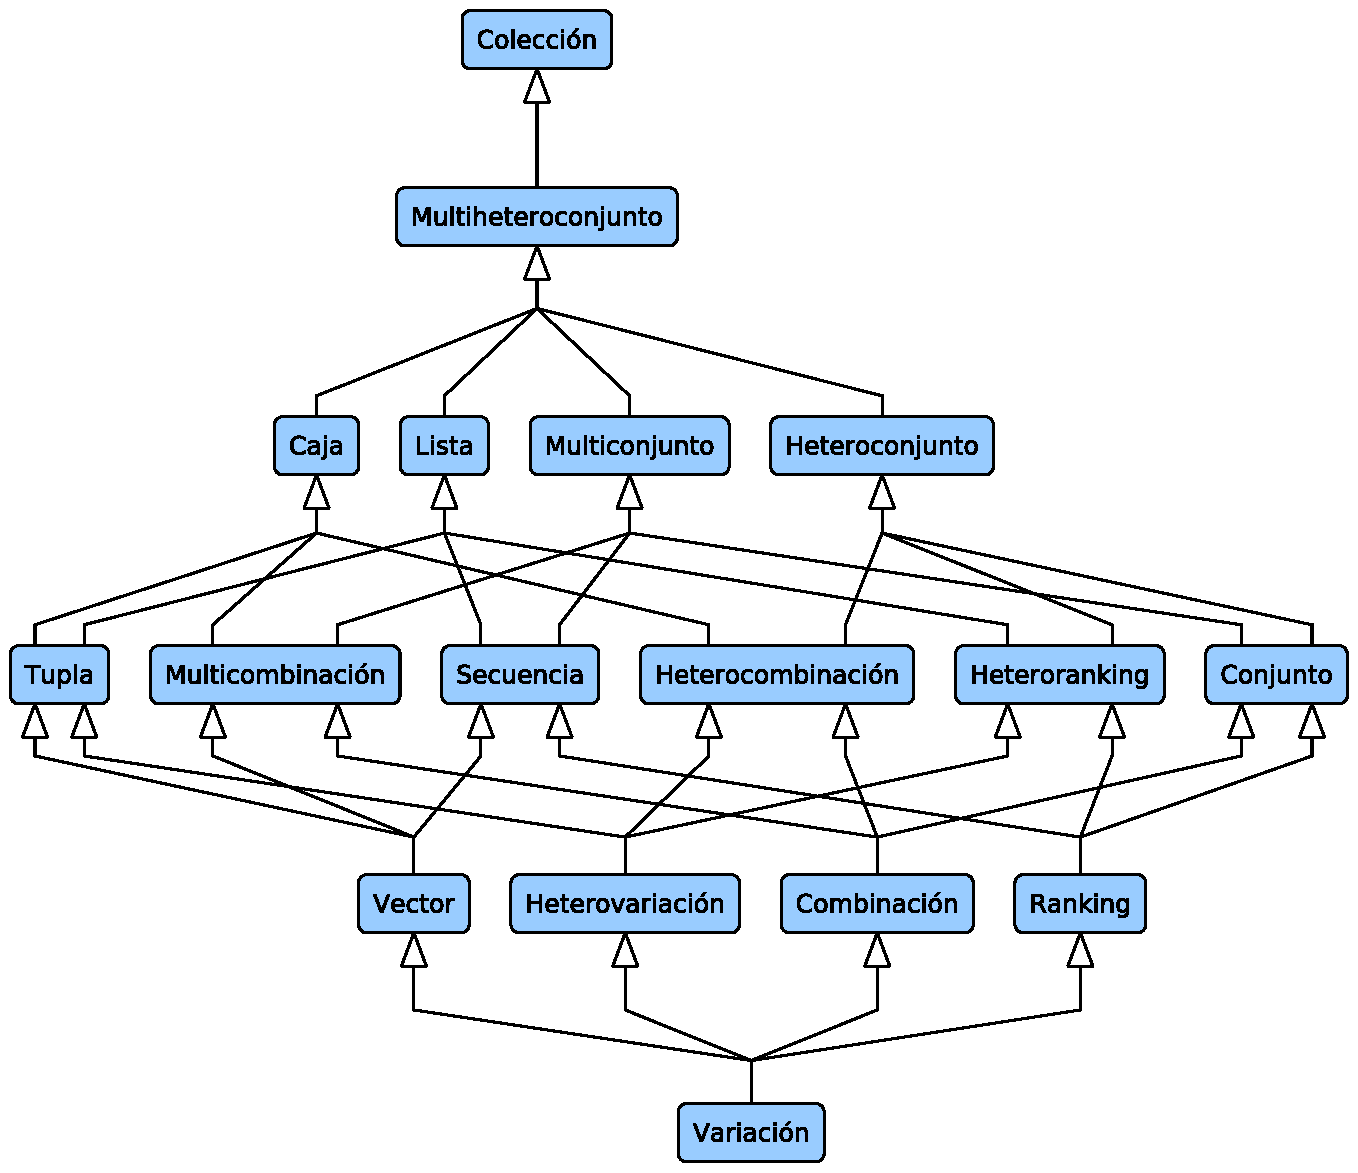
\includegraphics[width=\textwidth]{img/taxonomia_colecciones.pdf}
\figcaption{Taxonomía de colecciones.}
\label{fig:taxonomia-colecciones}
\end{center}
\end{figure} 

En la raíz de la taxonomía tenemos los \emph{multiheteroconjuntos}, que son las colecciones con menos restricciones estructurales, ya que son agrupaciones de elementos sin homogeneidad, sin unicidad, sin orden y sin cardinalidad fija.
Un ejemplo podría ser la bolsa de la compra en un supermercado ya que en la bolsa podemos poner elementos u objetos de distintos tipos (heterogeneidad), podemos poner objetos repetidos (sin unicidad), el orden de los objetos no importa (sin orden) y podemos poner cualquier número de objetos (cardinalidad variable).

En el extremo opuesto de la taxonomía están las \emph{variaciones}, que son las colecciones con más restricciones estructurales, ya que son homogéneas, con unicidad, con orden y con cardinalidad fija.
Este tipo de colecciones es bastante conocido en área de la combinatoria.

Entre estos dos tipos de de colecciones existen otros 14 tipos de colecciones en distintos niveles de la taxonomía según se apliquen más o menos restricciones sobre su estructura.
Algunas de estas colecciones bien conocidas por ser clásicos en distintas ramas de la Matemática, como los \emph{conjuntos}, las \emph{combinaciones}, los \emph{ranking}, las \emph{tuplas} o los \emph{vectores}, aunque estos últimos suelen limitarse a elementos numéricos.

Dados $n$ universos de elementos $E_1,\ldots, E_n$, sea $\cup E_i=\{E_1\cup \cdots\cup E_n\}$ la unión de los universos.
Dependiendo de las características estructurales de las colecciones se pueden definir las siguientes operaciones lógicas: 

\begin{description}
\item[Multiplicidad] La \emph{multiplicidad} o \emph{frecuencia} de un elemento $e$ en una colección $A$ es el número de veces que el elemento $x$ está contenido en $A$, es decir, el número de veces que se repite, y se denota $f_A(x)$. 

En general $f_A(x)\in \mathbb{Z}_{\geq 0}$ aunque en el caso de colecciones con unicidad $f_A(x)\in \{0,1\}$.

\item[Cardinalidad] El \emph{cardinal} de una colección $A$, que se denota $|A|$, es el número de elementos que contiene, es decir, $|A|=\sum_{x\in\cup E_i}f_A(x)$.

En el caso de colecciones con cardinalidad fija, todas las colecciones de ese tipo tendrán el mismo número de elementos.

\item[Pertenencia] Un elemento $x$ \emph{pertenece} a una colección $A$, y se denota $x\in A$, si y solo si $f_A(x)>0$.

\item[Inclusión] Una colección $A$ está \emph{incluida} en otra $B$, y se denota $A\subseteq B$, si $f_A(x)\leq f_B(x)$ $\forall x\in \cup E_i$.

\item[Suma] La \emph{suma} de dos colecciones sin unicidad $A$ y $B$, que se denota $A\uplus B$, es la colección formada por los elementos de $A$ y $B$ sumando sus multiplicidades, es decir, $f_{A\uplus B}(x)=f_A(x)+f_B(x)$ $\forall x\in \cup E_i$. 

Esta operación no tiene sentido para colecciones con unicidad.

\item[Unión] La \emph{unión} de dos colecciones $A$ y $B$, que se denota $A\cup B$, es la colección formada por los elementos de $A$ o $B$ con su máxima multiplicidad, es decir, $f_{A\cup B}(x)=\max\{f_A(x),f_B(x)\}$ $\forall x\in \cup E_i$.

\item[Intersección] La \emph{intersección} de dos colecciones $A$ y $B$, que se denota $A\cap B$, es el la colección formada por los elementos comunes de $A$ y $B$ con su mínima multiplicidad, es decir, $f_{A\cap
B}(x)=\min\{f_A(x),f_B(x)\}$ $\forall x\in \cup E_i$.

\item[Diferencia] La \emph{diferencia} de dos colecciones $A$ y $B$, que se denota $A-B$, es la colección que resulta de eliminar de $A$ los elementos de $B$, teniendo en cuentas sus multiplicidades, es decir,
$f_{A-B}(x)=\max\{f_A(x)-f_B(x),0\}$ $\forall x\in \cup E_i$.

\item[Complementario] La colección \emph{complementaria} de una colección con unicidad $A$, que se denota $\overline A$, es la colección formada por los elementos de $\cup E_i$ que no pertenecen a $A$, es decir, $f_{\overline A}(x)=1-f_A(x)$ $\forall x\in \cup E_i$.

Esta operación no tiene sentido para colecciones sin unicidad.

\item[Elemento $i$-ésimo] El \emph{elemento $i$-ésimo} de una colección con orden $A$, $i\leq |A|$, es el elemento que ocupa la posición $i$, y se denota $A[i]$.

Esta operación no tiene sentido para colecciones sin orden.

\item[Porción] La \emph{porción} de una colección con orden $A$ desde la posición $i$ hasta la posición $j$, $i\leq j\leq |A|$, que se denota $A[i,j]$, es la colección formada por los elementos de $A$ que ocupan las posiciones desde la $i$ hasta la $j$, es decir, $A[i,j]=[A[i],A[i+1],\ldots,A[j]]$.

Esta operación no tiene sentido para colecciones sin orden. 

\item[Concatenación] La \emph{concatenación} de las colecciones con orden $A$ y $B$, que se denota $A+B$, es la lista formada por los elementos de $A$ seguidos de los elementos de $B$, es decir, $A+B=[A[1],\ldots,a[|A|],B[1],\ldots,B[|B|]$.

Esta operación no tiene sentido para colecciones sin orden.

\item[Subcolección] Una colección con orden $A$ es una \emph{subcolección} de otra $B$, que se denota $A\sqsubseteq B$, si existe una secuencia creciente de enteros $i_k$, $k=1,\ldots,|A|$, tal que $A[k]=B[i_k]$.

Esta operación no tiene sentido para colecciones sin orden.

\item[Subcolección consecutiva] Una colección con orden $A$ es una \emph{subcolección consecutiva} de otra $B$, que se denota $A\preceq B$ si existen colecciones con orden tales que $B=C+A+D$.
Se cumple además que existen $i\leq j\leq |B|$ tales que $A=B[i,j]$.

Esta operación no tiene sentido para colecciones sin orden.
\end{description}


\section{Comparación de colecciones}

Al igual que cualquier otro proceso de comparación, la comparación de colecciones se realiza a través del estudio de las similitudes o diferencias entre los elementos que las componen por medio de funciones de similitud o disimilitud.

\subsection{Funciones de similitud}

\begin{definition}[Función de similitud]
Dado un conjunto $E$ de elementos, una \emph{función de similitud} es una función $\sigma:E\times
E \longrightarrow \mathbb{R}^+$ que asocia a cada par de elementos de $E$ un número real que expresa el grado de parecido entre dichas elementos y que cumple los siguientes axiomas:
\begin{align*}
    \textrm{No negatividad: }& \forall x,y \in E,\ \sigma(x,y)\geq 0,\\
    \textrm{Maximalidad: }& \forall x,y \in E,\ \sigma(x,x)\geq \sigma(x,y).
\end{align*}
\end{definition}

Algunos autores añaden a estas propiedades la propiedad de \emph{simetría}:
\[\forall x,y\in E, \sigma(x,y) = \sigma(y,x).\]
No obstante, tal y como refleja \cite{tversky1977features}, existen situaciones en determinados contextos en las que esta propiedad no se cumple y por tanto no se ha incluido en la definición anterior.

El ejemplo más trivial de función de similitud es la función de similitud identidad, que sirve para cualquier tipo de dato. 

\begin{definition}[Función de similitud identidad]
Dado un universo $E$ de elementos de cualquier tipo de datos, la \emph{función de similitud identidad} es una función de similitud \mbox{$\sigma_{id}: E\times E\longrightarrow [0,1]$} tal que
\[
\sigma_{id}(s,t)=
\begin{cases}
1, & \text{si $s=t$}; \\
0, & \text{si $s\neq t$}. 
\end{cases}
\]
\end{definition}

De igual modo que se define una función de similitud se puede definir una función de disimilitud:
\begin{definition}[Función de disimilitud]
Dado un conjunto $E$ de elementos, una \emph{función de disimilitud} es una función $\delta:E\times E \longrightarrow
\mathbb{R}^+$ que asocia a cada par de elementos de $E$ un número real que expresa el grado de diferencia entre dichas elementos y que cumple los siguientes axiomas:
\begin{align*}
    \textrm{No negatividad: }& \forall x,y \in E,\ \delta(x,y)\geq 0,\\
    \textrm{Minimalidad: }& \forall x \in E,\ \delta(x,x)=0.
\end{align*}
\end{definition}

En ocasiones se suelen utilizar definiciones más restringidas de funciones de disimilitud como son las distancias o métricas.

\begin{definition}[Distancia]
Dado un conjunto $E$ de elementos, una \emph{distancia} es una función de disimilitud que además cumple los siguientes axiomas:
\begin{align*}
    \textrm{Coincidencia: } & \forall x,y \in E,\ \delta(x,y)= 0\textrm{ si y solo si  }x=y,\\
    \textrm{Simetría: } & \forall x,y \in E,\ \delta(x,y) = \delta(y,x),\\
    \textrm{Desigualdad triangular: }& \forall x,y,z \in E,\ \delta(x,y)+\delta(y,z)\geq \delta(x,z).
\end{align*}
\end{definition}

Habitualmente las funciones de similitud o disimilitud suelen normalizarse, restringiendo su rango al intervalo real $[0,1]$ para facilitar la comparación entre distintas medidas.

\begin{definition}[Función de similitud normalizada]
Se dice que una función de (di)similitud está \emph{normalizada} si su rango es el intervalo real $[0,1]$.
\end{definition}

La mayoría de las funciones de similitud que se presentan en este artículo son funciones normalizadas, como por ejemplo la función de similitud identidad, aunque cuando pueda haber dudas, se utilizará la notación $\overline{\sigma}$ y $\overline{\delta}$ para distinguir las versiones normalizadas de las no normalizadas $\sigma$ y $\delta$ respectivamente.

Muy a menudo, las funciones de similitud se construyen a partir de funciones de disimilitud o distancias.

\begin{definition}[Correspondencia entre funciones de similitud y disimilitud]
Dada una función de similitud normalizada $\overline\sigma:E\times E \longrightarrow [0,1]$, y una función de disimilitud $\delta:E\times E \longrightarrow \mathbb{R}$, diremos que $\overline\sigma$ y $\delta$ se
\emph{corresponden}, si 
\[ \overline\sigma(x,y) = \pi(\delta(x,y)), \] 
para algún isomorfismo $\pi: R \longrightarrow [0,1]$ que invierta el orden (monótono decreciente) y tal que $\pi(0)=1$.
\end{definition}

Algunos isomorfismos habituales para $\pi$ son:
\begin{itemize}
\item $\pi(x)=1-x$, cuando $\delta$ está normalizada.
\item $\pi(x)=1-\dfrac{x}{\max \delta}$, cuando $\delta$ tiene un valor máximo.
\item $\pi(x)=1-\dfrac{x}{1+x}$, cuando $\delta$ no está acotada.
\end{itemize}

Uno de los principales problemas en un proceso de comparación es seleccionar las funciones de similitud apropiadas al contexto en el que se realizan las comparaciones. 
En el caso de la comparación de colecciones hay que tener en cuenta las propiedades estructurales del tipo de colecciones que se quieren comparar.  

En las próximas secciones se presenta un catálogo de funciones de similitud o disimilitud para los tipos colecciones identificados en la sección~\ref{sec:taxonomia-colecciones}.
Las funciones de este catálogo se han organizado siguiendo la misma clasificación taxonómica de colecciones allí definida. 
De esta manera, es trivial determinar las funciones de similitud que pueden utilizarse para comparar dos colecciones sin más que saber el tipo al que pertenecen.
Otra ventaja de la organización taxonómica es que se pueden comparar incluso colecciones de distintos tipos, utilizando las funciones de similitud de los tipos de colecciones que son ancestros comunes en la taxonomía de colecciones.

Sin duda, esta catalogación puede ayudar al usuario a seleccionar las funciones de similitud más apropiadas y también puede facilitar la definición de reglas de aplicación que automaticen el proceso de comparación,
como por ejemplo la aplicación de funciones de similitud en cascada.


\subsection{Catálogo de funciones de similitud}

\subsubsection{Funciones de similitud para multiheteroconjuntos}
\label{sec:sim-multiheteroconjuntos}

Los multiheteroconjuntos son las colecciones menos estructuradas ya que no tienen restricciones sobre la homogeneidad, la cardinalidad, el orden o la unicidad.
Esto dificulta su comparación, especialmente cuando los elementos que los componen son incomparables, y por tanto, las funciones
de similitud para compararlos son poco precisas.
La medida de similitud más simple para multiheteroconjuntos surge de la comparación de sus cardinalidad.

\begin{definition}[Función de similitud de cardinalidad]
Dados dos multiheteroconjuntos $A$ y $B$, la \emph{función de similitud de cardinalidad} es una función de similitud se define como 
\[
\sigma(A,B)= 1-\frac{||A|-|B||}{\max\{|A|,|B|\}}.
\]
\end{definition}

\begin{example}[Función de similitud de cardinalidad]
Dados los multiheteroconjuntos $A=\{1,1,2,\allowbreak 2,3,4,a,a,b\}$ y $B=\{1,3,3,4,4,4,a,a,a,a,c\}$,
\[
\sigma(A,B) = 1 - \frac{||A|-|B||}{\max\{|A|,|B|\}} = 1-\frac{|9-11|}{\max\{9,11\}} = 1- \frac{2}{11} = 0.82.
\]
\end{example}

Esta función de similitud solo tiene en cuenta el número de elementos en los multiheteroconjuntos, pero no su contenido.
Es posible precisar más la similitud teniendo en cuenta los elementos comunes y sus repeticiones en los multiheteroconjuntos.
Con este enfoque, la función de similitud más intuitiva que surge es la propuesta en \cite{jaccard1901etude} y que resulta de comparar la intersección y la unión.

\begin{definition}[Función de similitud de Jaccard]
Dados dos multiheteroconjuntos $A$ y $B$, la \emph{función de similitud de Jaccard} se define como
\[
\sigma(A,B)=\frac{|A\cap B|}{|A\cup B|}.
\]
\end{definition}

\begin{example}[Función de similitud de Jaccard]
Dados los multiheteroconjuntos $A=\{1,1,2,\allowbreak 2,3,4,a,a,b\}$ y $B=\{1,3,3,4,4,4,a,a,a,a,c\}$,
\[
\sigma(A,B)=\frac{|A\cap B|}{|A\cup B|} = \frac{|\{1,3,4,a,a\}|}{|\{1,1,2,2,3,3,4,4,4,a,a,a,a,b,c\}|} \frac{5}{15} = 0.33.
\]
\end{example}

Otra función de similitud más optimista que utiliza este mismo enfoque se propone en \cite{braunblanquet1932plant}, y compara la intersección con el mayor de los dos conjuntos, en lugar de con la unión. 

\begin{definition}[Función de similitud de Braun-Blanquet]
Dados dos multiheteroconjuntos $A$ y $B$, la \emph{función de similitud de Braun-Blanquet} se define como
\[
\sigma(A,B)=\frac{|A\cap B|}{\max\{|A|,|B|\}}.
\]
\end{definition}

\begin{example}[Función de similitud de Braun-Blanquet]
Dados los multiheteroconjuntos $A=\{1,1,2,\allowbreak 2,3,4,a,a,b\}$ y $B=\{1,3,3,4,4,4,a,a,a,a,c\}$,
\[
\sigma(A,B)=\frac{|A\cap B|}{\max\{|A|,|B|\}} = \frac{5}{11} = 0.45.
\]
\end{example}

Más optimista aún es la función de similitud de \cite{simpson1960notes}, que compara la intersección con el menor de los dos conjuntos. 

\begin{definition}[Función de similitud de Simpson]
Dados dos multiheteroconjuntos $A$ y $B$, la \emph{función de similitud de Simpson} se define como
\[
\sigma(A,B)=\frac{|A\cap B|}{\min\{|A|,|B|\}}.
\]
\end{definition}

\begin{example}[Función de similitud de Simpson]
Dados los multiheteroconjuntos $A=\{1,1,2,\allowbreak 2,3,4,a,a,b\}$ y $B=\{1,3,3,4,4,4,a,a,a,a,c\}$,
\[
\sigma(A,B)=\frac{|A\cap B|}{\min\{|A|,|B|\}}. = \frac{5}{9} = 0.55.
\]
\end{example}

Entre la medida de similitud de Braun-Blanquet y la de Simpson existe todo un repertorio de funciones de similitud que comparan el número de elementos de la  intersección con un número entre la cardinalidad de $A$ y la de $B$, como por ejemplo las funciones de similitud de \cite{dice1945measures}, \cite{ochiai1957zoogeographical} y \cite{kulczynski1927pflanzenassoziationen} que toman la media aritmética, geométrica y armónica del número de elementos de $A$ y $B$, respectivamente.
 
\begin{definition}[Función de similitud de Dice]
Dados dos multiheteroconjuntos $A$ y $B$, la \emph{función de similitud de Dice} se define como
\[
\sigma(A,B) = \frac{|A\cap B|}{\frac{|A|+|B|}{2}} = \frac{2|A\cap B|}{|A|+|B|}.
\]
\end{definition}

\begin{example}[Función de similitud de Dice]
Dados los multiheteroconjuntos $A=\{1,1,2,2,3,4,\allowbreak a,a,b\}$ y $B=\{1,3,3,4,4,4,a,a,a,a,c\}$,
\[
\sigma(A,B) = \frac{2|A\cap B|}{|A|+|B|} = \frac{2\cdot 5}{9+11} = 0.5.
\]
\end{example}

\begin{definition}[Función de similitud de Ochiai]
Dados dos multiheteroconjuntos $A$ y $B$, la \emph{función de similitud de Ochiai} se define como
\[
\sigma(A,B) = \frac{|A\cap B|}{\sqrt{|A||B|}}.
\]
\end{definition}

\begin{example}[Función de similitud de Ochiai]
Dados los multiheteroconjuntos $A=\{1,1,2,2,3,4,\allowbreak a,a,b\}$ y $B=\{1,3,3,4,4,4,a,a,a,a,c\}$,
\[
\sigma(A,B) = \frac{|A\cap B|}{\sqrt{|A||B|}} = \frac{5}{\sqrt{9\cdot11}} = 0.5.
\]
\end{example}

\begin{definition}[Función de similitud de Kulczynski]
Dados dos multiheteroconjuntos $A$ y $B$, la \emph{función de similitud de Kulczynski} se define como
\[
\sigma(A,B) = \frac{|A\cap B|}{\frac{2}{\frac{1}{|A|}+\frac{1}{|B|}}} = \frac{1}{2}\left(\frac{|A\cap B|}{|A|}+\frac{|A\cap B|}{|B|} \right).
\]
\end{definition}

\begin{example}[Función de similitud de Kulczynski]
Dados los multiheteroconjuntos $A=\{1,1,2,\allowbreak 2,3,4,a,a,b\}$ y $B=\{1,3,3,4,4,4,a,a,a,a,c\}$,
\[
\sigma(A,B) = \frac{1}{2}\left(\frac{|A\cap B|}{|A|}+\frac{|A\cap B|}{|B|} \right) =
\frac{1}{2}\left(\frac{5}{9}+\frac{5}{11} \right) = 0.5.
\]
\end{example}

Otra función de similitud más general, utilizada habitualmente en el campo de la Recuperación de Información, que también puede extenderse fácilmente a la comparación de multiconjuntos es la medida F \cite{rijsbergen1979information}.
En el ámbito de la Recuperación de la Información, cuando se quiere comparar un conjunto de resultados obtenidos $A$ con
el conjunto de los resultados que debería obtenerse $B$, se utilizan habitualmente dos medidas conocidas como
\emph{precisión} y \emph{exhaustividad}, que se definen de la siguiente manera
\begin{align*}
\mbox{Precisión } P &= \frac{|A\cap B|}{|A|},\\
\mbox{Exhaustividad } E&= \frac{|A\cap B|}{|B|},
\end{align*}
y la medida F se define como la media armónica ponderada entre ellas
\[
F = \frac{1}{\alpha\frac{1}{P}+(1-\alpha)\frac{1}{E}}=\frac{(1+\beta^2)P\,E}{\beta^2 P+E}, \mbox{con }
\beta^2=\frac{1-\alpha}{\alpha}
\]
donde $\alpha\in[0,1]$ y $\beta^2\in [0,\infty]$.

Su extensión a multiheteroconjuntos da lugar a la siguiente medida de similitud. 

\begin{definition}[Función de similitud F]
Dados dos multiheteroconjuntos $A$ y $B$, la \emph{función de similitud F} se define como
\[
\sigma_\beta(A,B) = \frac{(1+\beta^2)|A\cap B|}{|A|+\beta^2|B|}.
\]
donde $\beta\in \mathbb{R}^+.$
\end{definition}

Esta función no es simétrica ya que para $\beta<1$ se da más importancia a $A$ y para $\beta>1$ se da más importancia $B$. 
El único caso en que es simétrica es para $\beta=1$ y en ese caso se obtiene la función de similitud de Dice.

\begin{example}[Función de similitud F]
Dados los multiheteroconjuntos $A=\{1,1,2,2,3,4,a,a,b\}$ y $B=\{1,3,3,4,4,4,a,a,a,a,c\}$, y tomando $\beta=0.5$, se tiene
\[
\sigma_{0.5}(A,B) = \frac{(1+0.5^2)|A\cap B|}{|A|+0.5^2|B|} = \frac{1.25\cdot 5}{9+0.25\cdot 11} = 0.53.
\]
Mientras que tomando $\beta=2$ se tiene
\[
\sigma_{2}(A,B) = \frac{(1+2^2)|A\cap B|}{|A|+2^2|B|} = \frac{5\cdot 5}{9+4\cdot 11} = 0.47.
\]
\end{example}

En general, casi todas estas funciones de similitud se derivan de dos familias. 
La primera se debe a \cite{caillez1996contribution}.

\begin{definition}[Función de similitud de Caillez-Kuntz]
Dados dos multiheteroconjuntos $A$ y $B$, la \emph{función de similitud de Caillez-Kuntz} se define como
\[
\sigma_\alpha(A,B) = \frac{|A\cap B|}{\sqrt[\alpha]{\frac{|A|^\alpha+|B|^\alpha}{2}}}.
\]
donde $\alpha\in \mathbb{R}$.
\end{definition}

De esta familia se obtienen algunas de las funciones anteriores para distintos valores de $\alpha$.
Por ejemplo, para $\alpha=-\infty$ se obtiene la función de similitud de Simpson, para $\alpha=-1$ la función de similitud de Kulczynski, para $\alpha=0$ la función de similitud de Ochiai, para $\alpha=1$ la función de similitud de Dice y para $\alpha=\infty$ la función de similitud de Braun-Blanquet.

La segunda familia de funciones se debe a \cite{gower1986metric}.

\begin{definition}[Función de similitud de Gower-Legendre]
Dados dos multiheteroconjuntos $A$ y $B$, la \emph{función de similitud de Gower-Legendre} se define como
\[
\sigma_\eta(A,B) = \frac{\eta|A\cap B|}{|A|+|B|+(\eta-2)|A\cap B|}.
\]
donde $\eta\in \mathbb{R}$.
\end{definition}

De esta familia también se obtienen algunas de las funciones anteriores para distintos valores de $\eta$, como por ejemplo la función de similitud de Jaccard para $\eta=1$ o la función de similitud de Dice para $\eta=2$. 

Otra familia de funciones de similitud aún más general surge del modelo de ratio de Tversky \cite{tversky1977features}, donde las similitudes entre dos objetos $A$ y $B$ dependen de las características comunes a $A$ y $B$, las características de $A$ que no tiene $B$ y las características de $B$ que no tiene $A$.
Esto puede traducirse a multiheteroconjuntos como los elementos comunes a $A$ y $B$, es decir $A\cap B$; los elementos en $A$ que no están en $B$, es decir $A-B$; y los elementos en $B$ que no están en $A$, $B-A$.
Estos multiheteroconjuntos aparecen representados gráficamente en la figura~\ref{fig:multiheteroconjuntos-tversky}.

\begin{figure}[htp]
\begin{center}
\begin{tikzpicture}
\tikzset{venn circle/.style={draw,circle,minimum width=4cm,fill=#1,opacity=0.4}}
% Nodos
\node [rectangle, draw, minimum width=7cm, minimum height=5cm] at (1,0) {};
\node [venn circle = color1] (A) at (0,0) {};
\node at (-1,0) {$A-B$};
\node [venn circle = color2] (B) at (0:2cm) {};
\node at (3,0) {$B-A$};
\node at (barycentric cs:A=1/2,B=1/2 ) {$A \cap B$};
\node at (-1,-2cm) {$A$};
\node at (3,-2cm) {$B$};
\end{tikzpicture}
\figcaption{Multiheteroconjuntos involucrados en la comparación de dos multiheteroconjuntos $A$ y $B$ según el modelo de contraste de Tversky.}
\label{fig:multiheteroconjuntos-tversky}
\end{center}
\end{figure}


\begin{definition}[Función de similitud de Tversky]
Dados dos multiheteroconjuntos $A$ y $B$, la \emph{función de similitud de Tversky} se define como
\[
\sigma_{\beta,\gamma} (A,B) = \frac{|A\cap B|}{|A\cap B|+\beta |A-B|+\gamma |B-A|},
\]
donde $\beta,\gamma\in \mathbb{R}^+$ son pesos que le dan mayor o menor importancia a los elementos no comunes de ambos multiheteroconjuntos.
\end{definition}

Esta función de similitud no es simétrica si $\beta\neq \gamma$.
Esto tiene sentido si, al comparar los multiheteroconjuntos uno de ellos es considerado como referente \cite{tversky1977features}.
Cuando, por ejemplo, el segundo multiheteroconjunto se toma como referente, el peso de los elementos de $B$ que no están en $A$, debe ser más grande que el peso de los elementos en $A$ que no están $B$, de manera que $\beta<\gamma$.

\begin{example}[Función de similitud de Tversky]
Dados los multiheteroconjuntos $A=\{1,1,2,2,3,\allowbreak 4,a,a,b\}$ y $B=\{1,3,3,4,4,4,a,a,a,a,c\}$, y tomando $\beta=1$ y $\gamma=1$, se tiene
\[
\sigma(A,B) = \frac{|A\cap B|}{|A\cap B|+ |A-B|+ |B-A|} = \frac{5}{5+4+6} = \frac{5}{15} = 0.33.
\]
Si se toma como referente el segundo multiheteroconjunto, tomando por ejemplo $\beta=0.25$ y $\gamma=0.75$, entonces se tiene
\[
\sigma(A,B) = \frac{|A\cap B|}{|A\cap B|+ 0.25|A-B|+ 0.75|B-A|} = \frac{5}{5+0.25\cdot 4+0.75\cdot 6} = 0.48.
\]
que es diferente de la medida de similitud que obtiene al comparar $B$ con $A$
\[
\sigma(B,A) = \frac{|B\cap A|}{|B\cap A|+ 0.25|B-A|+ 0.75|A-B|} = \frac{5}{5+0.25\cdot 6+0.75\cdot 4} = 0.53.
\]
\end{example}

Dependiendo de los valores de $\beta$ y $\gamma$ se obtienen diferentes funciones de similitud.
Por ejemplo, para $\beta=\gamma=1$ se obtienen la función de similitud de Jaccard, y para $\beta=\gamma=1/2$, se obtiene la función de
similitud de Dice.
También se pueden deducir familias enteras de funciones de similitud como la función de similitud $F$, tomando
$\beta=1/(1+\beta'^2)$ y $\gamma=\beta'^2/(1+\beta'^2)$, donde $\beta'$ es el parámetro asociado a esta Función, o en general la familia de funciones de similitud en las que se cumple $\beta+\gamma=1$ \cite{rodrguez2003determining}.

Teniendo en cuenta las definiciones de estas familias de funciones de similitud, es posible definir otra familia más general aún que las engloba. 
Esta nueva función se ha llamado \emph{función de similitud de Tversky generalizada}.

\begin{definition}[Función de similitud de Tversky generalizada]
Dados dos multiheteroconjuntos $A$ y $B$, la \emph{función de similitud de Tversky generalizada} se define como
\[
\sigma_{\alpha,\beta,\gamma} (A,B) = \frac{|A\cap
B|}{\sqrt[\alpha]{\beta|A|^\alpha+\gamma|B|^\alpha+(1-\beta-\gamma)|A\cap B|^\alpha}},
\]
donde $\alpha\in \mathbb{R}$ y  $\beta,\gamma\in \mathbb{R}^+$.
\end{definition}

La demostración de que esta función de similitud engloba a las familias de funciones de similitud de Caillez-Kuntz, Gower-Legendre y Tverksy puede verse en \cite{sanchezalberca2015modelado}.

En la tabla~\ref{tab:tversky} se presenta un resumen de las funciones de similitud más comunes que resultan de instanciar la función de similitud de Tversky generalizada para diferentes valores de $\alpha$, $\beta$ y $\gamma$.

\begin{table}[htbp!]
\caption{Funciones de similitud para multiheteroconjuntos derivadas de la de Tversky.\label{tab:tversky}}
\[
\renewcommand*{\arraystretch}{1.5}
\begin{array}{lcccc}
\toprule
\text{\bf Similarity function} & \mbox{\boldmath$\alpha$} & \mbox{\boldmath$\beta$} & \mbox{\boldmath$\gamma$} &
\text{\bf Formula}\\
\midrule
\text{Jaccard} & 1 & 1 & 1 & \dfrac{|A\cap B|}{|A\cup B|}\\
\text{Braun-Blanquet} &+\infty & 0.5 & 0.5 & \dfrac{|A\cap B|}{\max\{|A|,|B|\}}\\
\text{Simpson} & -\infty & 0.5 & 0.5 & \dfrac{|A\cap B|}{\min\{|A|,|B|\}}\\
\text{Dice} & 1 & 0.5 & 0.5 & \dfrac{2|A\cap B|}{|A|+|B|}\\
\text{Ochiai} & 0 & 0.5 & 0.5 & \dfrac{|A\cap B|}{\sqrt{|A||B|}}\\
\text{Kulczynski} & -1 & 0.5 & 0.5 & \dfrac{1}{2}\left(\dfrac{|A\cap B|}{|A|}+\dfrac{|A\cap B|}{|B|} \right)\\
\text{Sokal-Sneath} & 1 & 2 & 2 & \dfrac{|A\cap B|}{2|A|+|2|B-3|A\cap B|}\\
\text{F} & 1 & 1/(1+\beta'^2) & \beta'^2/(1+\beta'^2) & \dfrac{(1+\beta'^2)|A\cap B|}{|A|+\beta'^2|B|}\\
\text{Rodríguez-Egenhofer} & 1 & 1-\gamma & \gamma & \dfrac{|A\cap B|}{\gamma |A|+(1-\gamma)|B|}\\
\bottomrule
\end{array}
\]
\end{table}

Disponer de una familia parametrizada de funciones de similitud no es sólo interesante desde el punto de vista de simplificar la implementación de todas ellas, sino también porque permite entender mejor la relación entre estas funciones de similitud, pero sobre todo porque permite generar nuevas funciones de similitud para distintas configuraciones de los parámetros. 
De hecho, esta nueva función de similitud abre la puerta a la experimentación para la determinación, mediante técnicas de aprendizaje automático, de la combinación de valores para los parámetros que dan mejores resultados en cada contexto de aplicación, disponiendo así de funciones de similitud a la carta. 

\subsubsection{Funciones de similitud para multiconjuntos}
\label{sec:sim-multiconjuntos}

En primer lugar, puesto que los multiconjuntos son un caso particular de los multiheteroconjuntos, es posible utilizar cualquiera de las funciones de similitud vistas en la sección~\ref{sec:sim-multiheteroconjuntos} para comparar multiconjuntos.

Por otro lado, puesto que los multiconjuntos pueden interpretarse como muestras con una distribución de frecuencias dada por las
multiplicidades de sus elementos, es posible utilizar funciones de similitud para comparar distribuciones de frecuencias, como por
ejemplo el test de la Chi-cuadrado \cite{manning1999foundations}.

\begin{definition}[Función de similitud Chi-cuadrado]
Dados dos multiconjuntos $A$ y $B$, la \emph{función de similitud Chi-cuadrado} se define como
\[
\sigma(A,B) = P(\chi^2(n)\geq \chi^2(A,B)),
\]
donde
\[
\chi^2(A,B)=\sum_{x\in A} \frac{(f_B(x)-f_A(x))^2}{f_A(x)},
\]
es el estadístico Chi-cuadrado para los multiconjuntos $A$ y $B$, y $\chi^2(n)$ es el valor de la función de distribución de una Chi-cuadrado con $n$ grados de libertad, siendo $n$ el número de elementos distintos de $A$ menos 1.
\end{definition}

\begin{example}[Función de similitud Chi-cuadrado]
Dados los multiconjuntos $A=\{a,a,b,\allowbreak c,d,d,e\}$ y $B=\{a,a,a,a,b,b,c,d\}$, los cálculos del estadístico Chi-cuadrado aparecen en la siguiente tabla 
\[
\begin{array}{lccc}
\toprule
x & f_A(x) & f_B(x) & \frac{(f_B(x)-f_A(x))^2}{f_A(x)} \\
\midrule
a & 2 & 4 & 2\\
b & 1 & 2 & 1\\
c & 1 & 1 & 0\\
d & 2 & 1 & 0.5 \\
e & 1 & 0 & 1\\
\midrule
\sum & & & 4.5\\
\bottomrule
\end{array}
\]
con lo que se tiene
\[
\sigma(A,B) = P(\chi^2(4)\geq 4.5) = 0.343,
\]
\end{example}

Obsérvese que esta medida de similitud no es simétrica y además no puede calcularse cuando alguno de los elementos del segundo multiconjunto tiene multiplicidad 0.
En tal caso podría utilizarse test exacto de Fisher. 

Un enfoque diferente consiste en asignar un peso a cada elemento que depende no solo de la multiplicidad en el multiconjunto, sino también de su multiplicidad en otros multiconjuntos del mismo dominio de aplicación.
Una función bien conocida que utiliza este enfoque es la Frecuencia de Términos $\times$ Frecuencia Inversa de
Documentos, más conocida como TF$\times$IDF (del inglés Term Frequency $\times$ Inverse Document Frequency).
Esta función se aplica habitualmente en el modelo de espacio de vectores para comparar documentos, vistos como multiconjuntos de palabras \cite{salton1975vector}. 
La idea consiste en cuantificar la importancia de un término en un documento teniendo en cuenta su frecuencia dentro del documento y fuera de él en un corpus de documentos de referencia. 
La importancia del término aumenta a medida que su frecuencia aumenta en el documento, y disminuye a medida que su frecuencia aumenta en el corpus. 

\begin{definition}[TF$\times$IDF]
Dados un multiconjunto $A$ y un corpus de multiconjuntos $\mathcal{C}$ en el mismo universo, se define la función
\[
\textrm{TF}\times\textrm{IDF}_{A,\mathcal{C}}(x)=f_A(x)\log(|\mathcal{C}|/|\mathcal{C}(x)|),
\]
donde $\mathcal{C}(x)$ es el subconjunto de multiconjuntos de $\mathcal{C}$ que contienen el término $x$.
\end{definition}

La base del logaritmo no es importante aunque habitualmente suele tomarse 2.

Para definir la función de similitud para multiconjuntos basada en la función TF$\times$IDF, un multiconjunto $A$ es considerado como un vector donde cada dimensión corresponde a un elemento del universo de los multiconjuntos $E=\{x_1,\ldots,x_n\}$, y la
componente $i$ es el peso del elemento $x_i$ en el multiconjunto, es decir, TF$\times$IDF$_{A,\mathcal{C}}(x_i)$.
Con estos vectores, la similitud entre multiconjuntos puede calcularse con cualquiera de las distancias en el espacio Euclideo $n$ dimensional, como por ejemplo, la distancia Euclidea, el producto escalar o el coseno (ver
sección~\ref{sec:sim-vectores}).

\begin{definition}[Función de similitud TF$\times$IDF]
Dados dos multiconjuntos $A$ y $B$, y un corpus de multiconjuntos $\mathcal{C}$ en el mismo universo, la \emph{función de
similitud TF$\times$IDF} se define como
\[
\sigma_{\mathcal{C}}(A,B)=
\frac{\sum_{i=1}^{n}\textrm{TF}\times\textrm{IDF}_{A,\mathcal{C}}(x_i)\cdot \textrm{TF}\times\textrm{IDF}_{B,\mathcal{C}}(x_i)}
{\sqrt{\sum_{i=1}^n (\textrm{TF}\times\textrm{IDF}_{A,\mathcal{C}}(x_i))^2 \cdot \sum_{i=1}^n (\textrm{TF}\times\textrm{IDF}_{B,\mathcal{C}}(x_i))^2}}
\]
\end{definition}

% \begin{example}[Función de similitud TF$\times$IDF]
% Para ilustrar el cálculo de esta función de similitud hemos considerado un corpus de 20 ácidos comunes:
% $\mathcal{C}=\{$HF, HCl, HBr, HI, H$_2$S, HNO$_3$, HNO$_2$, HClO, HClO$_2$, HClO$_3$, HClO$_4$, H$_2$SO$_4$,
% H$_2$SO$_3$, H$_3$PO$_4$, H$_3$PO$_3$, H$_2$CO$_3$, HC$_2$H$_3$O$_2$, H$_2$C$_2$O$_4$, H$_3$BO$_3$, H$_2$SiO$_3$\}.
% Con este corpus se ha calculado la función TF$\times$IDF del HNO$_3$ (ácido nítrico), H$_2$CO$_3$ (ácido carbónico) y
% HC$_2$H$_3$O$_2$ (ácido acético); los detalles del cálculo se presentan en la tabla~\ref{tab:tf-idf-acids}. 
% La similitud TF$\times$IDF entre estos ácidos es
% {\footnotesize
% \begin{align*}
% \sigma_{\mathcal{C}}(\text{HNO$_3$};\text{H$_2$CO$_3$}) &=
% \frac{(0;1.25;0;0;0;3.32;0;0;0;0;0;0)\cdot(0;1.25;0;2.73;0;0;0;0;0;0;0;0)}
% {||(0;1.25;0;0;0;3.32;0;0;0;0;0;0)||\cdot||(0;1.25;0;2.73;0;0;0;0;0;0;0;0)||}\\
% &=\frac{1.55}{3.55\cdot 3.01}= 0.14.\\
% \sigma_{\mathcal{C}}(\text{HC$_2$H$_3$O$_2$};\text{H$_2$CO$_3$}) &=
% \frac{(0;0.83;0;5.47;0;0;0;0;0;0;0;0)\cdot(0;1.25;0;2.73;0;0;0;0;0;0;0;0)}
% {||(0;0.83;0;5.47;0;0;0;0;0;0;0;0)||\cdot||(0;1.25;0;2.73;0;0;0;0;0;0;0;0)||}\\
% &=\frac{16.02}{5.54\cdot 3.01} = 0.96.
% \end{align*}
% }
% Como puede observarse el peso del hidrógeno en los vectores es 0 porque está presente en todos los ácidos, de manera que el hecho
% de que dos ácidos tengan en común hidrógeno lógicamente no aumenta su similitud.
% \end{example}

% \begin{table}[htbp]
% \centering
% \begin{tabular}{!{\color{color1}\vrule}l!{\color{color1}\vrule}rr!{\color{color1}\vrule}rr!{\color{color1}\vrule}rr!{\color{color1}\vrule}rr!{\color{color1}\vrule}}
% \arrayrulecolor{color1}
% \cline{2-9}
% \multicolumn{1}{c|}{} & \multicolumn{2}{c|}{Corpus} & \multicolumn{2}{c|}{HNO$_3$} & \multicolumn{2}{c|}{H$_2$C0$_3$} &
%  \multicolumn{2}{c|}{HC$_2$H$_3$0$_2$}\\ 
% \hline
% Elemento & & $df$ & $idf$ & $tf$ & $tf\times idf$ & $tf$ & & $tf\times idf$ & $tf$ & & $tf\times idf$\\
% \hline
% H & & 20 & 0 &   & 1 &  & 0 & 2 & 0      & 4 &  0\\
% O & & 15 & $0.42$ & 3 & $1.25$& 3 & $1.25$ & 2 & $0.83$\\
% Cl & &  5 &  & 2 &   & 0 &  & 0 & 0 & & 0      & 0 & & 0\\
% C & &  3 & $2.73$ & 0 & 0 &   & 1 & $2.73$ & 2 & $5.47$\\
% S & &  3 & $2.73$ & 0 & & 0 &   & 0 & & 0 &    & 0 & & 0\\
% N & &  2 & $3.32$ & & 1 & & $3.32$& & 0 & & 0      & 0 & 0\\
% P & &  2 & $3.32$ & 0 &  & 0 & & 0 & & 0 &    & 0 & & 0\\
% B & &  1 & $4.32$ & 0 &     0 & & 0 & & 0 &    & 0 & & 0\\
% Si & &  1 & $4.32$ & 0 &     0 & & 0 & & 0 &    & 0 & & 0\\
% F & &  1 & $4.32$ & 0 &     0 & & 0 & & 0 &    & 0 & & 0\\
% I & &  1 & $4.32$ & 0 &     0 & & 0 & & 0 &    & 0 & & 0\\
% Br & &  1 & $4.32$ & 0 &     0 & & 0 & & 0 &    & 0 & & 0\\
% \hline
% \end{tabular}
% \caption{Detalles del cálculo de la función TF$\times$IDF del HNO$_3$ (ácido nítrico),
% H$_2$CO$_3$ (ácido carbónico) y HC$_2$H$_3$O$_2$ (ácido acético). 
% El corpus utilizado es el conjunto de los ácidos comunes: 
% $\mathcal{C}=\{$HF, HCl, HBr, HI, H$_2$S, HNO$_3$, HNO$_2$, HClO, HClO$_2$, HClO$_3$, HClO$_4$, H$_2$SO$_4$,
% H$_2$SO$_3$, H$_3$PO$_4$, H$_3$PO$_3$, H$_2$CO$_3$, HC$_2$H$_3$O$_2$, H$_2$C$_2$O$_4$, H$_3$BO$_3$, H$_2$SiO$_3$\}}.
% \label{tab:tf-idf-acids}
% \end{table}


\subsubsection{Funciones de similitud para heteroconjuntos}
\label{sec:sim-heteroconjuntos}

Los heteroconjuntos son un caso particular de multiheteroconjuntos, de manera que pueden utilizarse todas las funciones de similitud de la sección~\ref{sec:sim-multiheteroconjuntos} para comparar heteroconjuntos.
Más allá de estas funciones, en la literatura científica no se han encontrado otras funciones que utilicen además la condición de unicidad específica de los heteroconjuntos.


\subsubsection{Funciones de similitud para listas}
\label{sec:sim-listas}

Las listas son un caso particular de multiheteroconjuntos, de manera que
pueden utilizarse todas las funciones de similitud de la sección~\ref{sec:sim-multiheteroconjuntos} para comparar listas. 

Por otro lado, la restricción de orden que incorporan las listas le da mayor semántica a la colección y puede aprovecharse en distintas estrategias de comparación de listas.
La estrategia más sencilla consiste en contar el número de elementos que coinciden en la misma posición de dos listas y fue propuesta en \cite{hamming1950errordetecting} para la detección de errores en la transmisión de cadenas de bits. 

\begin{definition}[Función de similitud de Hamming para listas]
Dadas dos listas $A$ y $B$, la \emph{función de similitud de Hamming} se define como
\[
\sigma(A,B)=\frac{\sum_{i=1}^{\min\{|A|,|B|\}}\sigma_{id}(A[i],B[i])}{\max\{|A|,|B|\}},
\]
donde $\sigma_{id}$ es la función de similitud identidad.
\end{definition}

\begin{example}[Función de similitud de Hamming]
Dadas las las listas $A=[a,b,c,a,d,c,a,b]$ y $B=[a,d,e,a,f,c,a,d,c,a,b]$, los elementos que coinciden en la misma posición aparecen sombreados en la siguiente tabla:

\[
\begin{array}{|l|c|c|c|c|c|c|c|c|c|c|c|}
\hline
\textrm{Posición} & 1 & 2 & 3 & 4 & 5 & 6 & 7 & 8 & 9 & 10 & 11\\
\hline
A & \cellcolor{gray!40}a & b & c & \cellcolor{gray!40}a & d & \cellcolor{gray!40}c & \cellcolor{gray!40}a & b & & & \\
\hline
B & \cellcolor{gray!40}a & d & e & \cellcolor{gray!40}a & f & \cellcolor{gray!40}c & \cellcolor{gray!40}a & d & c & a & b\\
\hline
\end{array}
\]

Por tanto, la similitud de Hamming de $A$ y $B$ es
\[
\sigma(A,B) = \frac{\sum_{i=1}^{\min\{|A|,|B|\}}\sigma_{id}(A[i],B[i])}{\max\{|A|,|B|\}} =
\frac{1+0+0+1+0+1+1+0}{\max\{8,11\}}=\frac{4}{11}=0.37.
\]
\end{example}

Esta función solo tiene en cuenta las coincidencias de elementos en la misma posición. 
Sin embargo, es posible considerar las coincidencias de elementos dentro de una ventana de un determinado tamaño.

\begin{definition}[Ventana de coincidencia]
Dadas dos listas $A$ y $B$, la \emph{ventana de coincidencia} de tamaño $k$, que se denota $\operatorname{match}(A,B,k)$, es el conjunto de pares de posiciones $(i,j)$, $1\leq i\leq |A|$ y $1\leq j\leq |B|$, tales
que
\begin{itemize}[noitemsep,label=--]
\item $A[i]=B[j]$,
\item $i-k\leq j\leq i+k$,
\item $\not \exists l<j$ con $(i,l)\in \operatorname{match}(A,B,k)$,
\item $\not \exists m<i$ con $(m,j)\in \operatorname{match}(A,B,k)$.
\end{itemize}

Los elementos correspondientes a las posiciones de match$(A,B,k)$ son una sublista de $A$ que se llama \emph{sublista de la ventana de coincidencia de tamaño $k$} y es
\[
\operatorname{lmatch}(A,B,k)= \{A[i]\ |\ \exists j \text{ tal que  } (i,j)\in \operatorname{match}(A,B,k)\}
\]
\end{definition}

\begin{example}[Ventana de coincidencia]
Dadas las listas $A=[a,b,c,a,d,c,a,b]$ y $B=[a,d,e,a,f,c,a,d,c,a,b]$, para una ventana de coincidencia de tamaño 4, se tienen las siguientes coincidencias

\begin{center}
\begin{tikzpicture}
% Nodes
\node(P){Posición};
\node(1)[right of = P]{1};
\node(2)[right of = 1]{2};
\node(3)[right of = 2]{3};
\node(4)[right of = 3]{4};
\node(5)[right of = 4]{5};
\node(6)[right of = 5]{6};
\node(7)[right of = 6]{7};
\node(8)[right of = 7]{8};
\node(9)[right of = 8]{9};
\node(10)[right of = 9]{10};
\node(11)[right of = 10]{11};
\node(A)[below = 1mm of P]{$A$:};
\node(a1)[right of = A]{$a$};
\node(a2)[right of = a1]{$b$};
\node(a3)[right of = a2]{$c$};
\node(a4)[right of = a3]{$a$};
\node(a5)[right of = a4]{$d$};
\node(a6)[right of = a5]{$c$};
\node(a7)[right of = a6]{$a$};
\node(a8)[right of = a7]{$b$};
\node(B)[below of = A]{$B$:};
\node(b1)[right of = B]{$a$};
\node(b2)[right of = b1]{$d$};
\node(b3)[right of = b2]{$e$};
\node(b4)[right of = b3]{$a$};
\node(b5)[right of = b4]{$f$};
\node(b6)[right of = b5]{$c$};
\node(b7)[right of = b6]{$a$};
\node(b8)[right of = b7]{$d$};
\node(b9)[right of = b8]{$c$};
\node(b10)[right of = b9]{$a$};
\node(b11)[right of = b10]{$b$};
% Arcs
\draw (a1) -- (b1);
\draw (a3) -- (b6);
\draw (a4) -- (b4);
\draw (a5) -- (b2);
\draw (a6) -- (b9);
\draw (a7) -- (b7);
\draw (a8) -- (b11);
\end{tikzpicture}
\end{center}

de manera que 
\[
\operatorname{match}(A,B,4) = \{(1,1),(3,6),(4,4),(5,2),(6,9),(7,7),(8,11)\}\]

Del mismo modo se puede comprobar que 
\[
\operatorname{match}(B,A,4) = \{(1,1),(2,5),(4,4),(6,3),(7,7),(9,6),(11,8)\}
\]

Obsérvese $B[8]=d$ no coincide con $A[5]$ ya que esta posición fue previamente emparejada con $B[2]$.  
\end{example}

Utilizando la ventana de coincidencia se puede definir la siguiente función de similitud.
 
\begin{definition}[Función de similitud de la ventana de coincidencia]
Dadas dos listas $A$ y $B$, la \emph{función de similitud de ventana de coincidencia} de tamaño $k$ se define como
\[
\sigma_k(A,B)=\frac{|\operatorname{match}(A,B,k)|}{\max\{|A|,|B|\}}.
\]
\end{definition}

\begin{example}[Función de similitud de la ventana de coincidencia]
Según las ventanas de coincidencia calculadas en el ejemplo anterior, la similitud de ventana de coincidencia de tamaño 4 para las listas $A=[a,b,c,a,d,c,a,b]$ y $B=[a,d,e,a,f,c,a,d,c,a,b]$ es
\[
\sigma_4(A,B) = \frac{|\operatorname{match}(A,B,4)|}{\max\{|A|,|B|\}} = \frac{7}{11} = 0.64.
\]
\end{example}

Una variación de esta función de similitud que también tiene en cuenta las transposiciones de elementos en la ventana de coincidencia se debe a \cite{jaro1989advances}.

\begin{definition}[Función de similitud de Jaro]
Dadas dos listas $A$ y $B$, la \emph{función de similitud de Jaro} se define como
\[
\sigma(A,B) =
\frac{1}{3}\left(\frac{|\operatorname{match}(A,B)|}{|A|}+\frac{|\operatorname{match}(A,B)|}{|B|}+\frac{|\operatorname{match}(A,B)|-|\operatorname{lmatch}(A,B)|}
{|\operatorname{match}(A,B)|}\right)
\]
donde $\operatorname{match}(A,B)=\operatorname{match}(A,B,\frac{\max\{|A|,|B|\}}{2}-1)$ (es decir, el tamaño de la ventana de
coincidencia es la mitad del tamaño de la mayor lista menos uno) y $\operatorname{lmatch}(A,B)$ es el número de elementos en
$\operatorname{lmatch}(A,B,\allowbreak \frac{\max\{|A|,|B|\}}{2}-1)$ que no coinciden con los elementos de $\operatorname{lmatch}(B,A,\frac{\max\{|A|,|B|\}}{2}-1)$ en la misma posición, dividido por 2.
\end{definition}

\begin{example}[Función de similitud de Jaro]
Considerando de nuevo las listas $A=[a,b,c,a,d,c,a,b]$ y $B=[a,d,e,a,f,c,a,d,c,a,b]$, el tamaño de la ventana de coincidencia es $\frac{\max\{|A|,|B|\}}{2}-1= 4$, que es el mismo tamaño de la ventana de coincidencia del ejemplo anterior. 
Teniendo en cuenta además los elementos que no aparecen en la misma posición de las sublistas correspondientes a las ventanas de coincidencia, que aparecen sombreadas en la siguiente tabla

\[
\begin{array}{|l|c|c|c|c|c|c|c|}
\hline
\textrm{lmatch}(A,B,4) & a & \cellcolor{gray!40}c & a & \cellcolor{gray!40}d & \cellcolor{gray!40}c & \cellcolor{gray!40}a & b\\
\hline
\textrm{lmatch}(B,A,4) & a & \cellcolor{gray!40}d & a & \cellcolor{gray!40}c & \cellcolor{gray!40}a & \cellcolor{gray!40}c & b\\
\hline 
\end{array}
\]

se concluye que la similitud de Jaro es
\begin{align*}
\sigma(A,B) &=
\frac{1}{3}\left(\frac{|\operatorname{match}(A,B)|}{|P|}+\frac{|\operatorname{match}(A,B)|}{|B|}+\frac{|\operatorname{match}(A,B)|-|\operatorname{lmatch}(A,B)|}
{|\operatorname{match}(A,B)|}\right) =\\
&= \frac{1}{3}\left(\frac{7}{8}+\frac{7}{11}+\frac{7-2}{7}\right) = 0.74. 
\end{align*}
\end{example}

Cuando se aplica a palabras de un lenguaje, se ha comprobado que esta función de similitud funciona muy bien para identificar errores ortográficos. 

Otra variación de esta función de similitud que da mayor peso a los prefijos comunes se debe a \cite{winkler1999state}.

\begin{definition}[Función de similitud de Jaro-Winkler]
Dadas dos listas $A$ y $B$, la \emph{función de similitud de Jaro-Winkler} se define como
\[
\sigma(A,B)=\sigma_J(A,B)+\alpha|\operatorname{prefix}(A,B)|(1-\sigma_J(A,B)),
\]
donde $\sigma_J(s,t)$ es la función de similitud de Jaro, $\operatorname{prefix}(A,B)$ es la sublista consecutiva de mayor tamaño que es prefijo común a $A$ y $B$, hasta un máximo de 4, y $\alpha$ es un factor de escalado (normalmente $0.1$).
\end{definition}

\begin{example}[Función de similitud de Jaro-Winkler]
Considerando de nuevo las listas $A=[a,b,c,a,d,c,a,b]$ y $B=[a,d,e,a,f,c,a,d,c,a,b]$, su similitud de Jaro-Winkler es
\begin{align*}
\sigma(A,B)&=\sigma_J(A,B)+0.1|\operatorname{prefix}(A,B)|(1-\sigma_J(A,B)) = \\
&=0.74 + 0.1\cdot 1\cdot (1-0.74) = 0.77.
\end{align*}
\end{example}

Aunque las funciones de similitud de Jaro y de Jaro-Winkler son válidas para listas, en realidad provienen del área de la vinculación de registros y se utilizan fundamentalmente con cadenas de caracteres, que son un caso particular de secuencias (ver sección~\ref{sec:sim-secuencias}).

Otra forma natural de comparar listas es por medio de sus sublistas, especialmente cuando el orden es tan importante como para no permitir transposiciones.
La comparación se hace comparando el tamaño de la mayor sublista común.

\begin{definition}[Función de similitud de la mayor sublista común]
Dadas dos listas $A$ y $B$, la \emph{función de similitud de la mayor sublista común} se define como
\[
\sigma(A,B) = \frac{2\max\{|C|:C\sqsubseteq A, C\sqsubseteq B\}}{|A|+|B|}
\]
\end{definition}

\begin{example}[Función de similitud de la mayor sublista común]
La mayor sublista común de las listas $A=[a,b,c,a,d,c,a,b]$ y $B=[a,d,e,a,f,c,a,d,c,a,b]$ es $[a,c,a,d,c,a,b]$, y por tanto, la similitud de la mayor
sublista común es
\[
\sigma(A,B) = \frac{2|[a,c,a,d,c,a,b]|}{|A|+|B|} = \frac{2\cdot 7}{8+11} = 0.74. 
\]
\end{example}

También se pueden considerar sublistas consecutivas en lugar de sublistas. 

\begin{definition}[Función de similitud de la mayor sublista consecutiva común]
Dadas dos listas $A$ y $B$, la \emph{función de similitud de la mayor sublista consecutiva común} se define como
\[
\sigma(A,B) = \frac{2\max\{|C|:C\preceq A, C\preceq B\}}{|A|+|B|}
\]
\end{definition}

\begin{example}[Función de similitud de la mayor sublista consecutiva común]
La mayor sublista consecutiva común de las listas $A=[a,b,c,a,d,c,a,b]$ y $B=[a,d,e,a,f,c,a,d,c,a,b]$ es $[c,a,d,c,a,b]$, y por tanto, la similitud de la mayor sublista consecutiva común es 
\[
\sigma(A,B) = \frac{2|[c,a,d,c,a,b]|}{|A|+|B|} = \frac{2\cdot 6}{8+11} =
0.63.
\]
\end{example}

Se pueden considerar también variaciones de esta función de similitud que solamente tengan en cuenta los prefijos y los sufijos de las listas.

\begin{definition}{Función de similitud del mayor prefijo común}
Dadas dos listas $A$ y $B$, la \emph{función de similitud del mayor prefijo común} se define como
\[
\sigma(A,B)=\frac{2\max\{|C|: A=C+A', B=C+B'\}}{|A|+|B|}
\]
\end{definition}

\begin{example}[Función de similitud del mayor prefijo común]
El mayor prefijo común de las listas $A=[a,b,c,a,d,c,a,b]$ y $B=[a,d,e,a,f,c,a,d,c,a,b]$ es $[a]$, y por tanto, la similitud del mayor prefijo común es
\[
\sigma(A,B)=\frac{2\cdot |[a]|}{|A|+|B|} = \frac{2\cdot 1}{8+11} = 0.11.
\]
\end{example}

\begin{definition}[Función de similitud del mayor sufijo común]
Dadas dos listas $A$ y $B$, la \emph{función de similitud del mayor sufijo común} se define como
\[
\sigma(A,B)=\frac{2\max\{|C|: A=A'+C, B=B'+C\}}{|A|+|B|}
\]
\end{definition}

\begin{example}[Función de similitud del mayor sufijo común]
El mayor sufijo común de las listas $A=[a,b,c,a,d,c,a,b]$ y $B=[a,d,e,a,f,c,a,d,c,a,b]$ es $[c,a,d,c,a,b]$, y por tanto, la similitud del mayor sufijo común es
\[
\sigma(A,B) = \frac{2|[c,a,d,c,a,b]|}{|A|+|B|} = \frac{2\cdot 6}{8+11} =
0.63.
\]
\end{example}

Por supuesto también se pueden idear funciones de similitud que combinen prefijos y sufijos. 


\subsubsection{Funciones de similitud para cajas}
\label{sec:sim-cajas}
Las cajas son un caso particular de multiheteroconjuntos, de manera que
pueden utilizarse todas las funciones de similitud de la sección~\ref{sec:sim-multiheteroconjuntos} para comparar cajas.
Más allá de estas funciones, en la literatura científica no se han encontrado otras funciones que utilicen además la condición de cardinalidad fija específica de las cajas. 


\subsubsection{Funciones de similitud para conjuntos}
\label{sec:sim-conjuntos}

Los conjuntos son un caso particular de multiconjuntos y de
heteroconjuntos, de manera que pueden utilizarse todas las funciones de similitud de las secciones~\ref{sec:sim-multiconjuntos} y \ref{sec:sim-heteroconjuntos} para comparar conjuntos.
Las funciones de similitud definidas en esas secciones solamente tienen en cuenta los elementos comunes y no comunes en los conjuntos; sin embargo, cuando los elementos son diferentes no se tienen en cuenta sus diferencias.
Si existe una función de similitud o disimilitud para los elementos del universo, es posible calcular la similitud entre dos conjuntos como una función de la similitud entre sus elementos.
Existen varias alternativas; la más optimista es tomar los dos elementos más similares.

\begin{definition}[Función de similitud de elementos máxima]
Dados dos conjuntos $A$ y $B$ definidos sobre un mismo universo $E$ y una función de similitud normalizada $\sigma_E$ para los elementos de $E$, la \emph{función de similitud de elementos máxima} se define como
\[
\sigma(A,B)=\max\{\sigma_E(x,y): x\in A, y\in B\}.
\]
\end{definition}

La opción más pesimista consiste en tomar los dos elementos menos similares

\begin{definition}[Función de similitud de elementos mínima]
Dados dos conjuntos $A$ y $B$ definidos sobre un mismo universo $E$ y una función de similitud normalizada $\sigma_E$ para los elementos de $E$, la \emph{función de similitud de elementos mínima} se define como
\[
\sigma(A,B)=\min\{\sigma_E(x,y): x\in A, y\in B\}.
\]
\end{definition}

El problema de las opciones más optimista y más pesimista es que solamente tienen en cuenta un par de elementos, los más similares y los menos, respectivamente.
En muchos casos es más razonable considerar la similitud entre todos los posibles pares.

\begin{definition}[Función de similitud de elementos media]
Dados dos conjuntos $A$ y $B$ definidos sobre un mismo universo $E$ y una función de similitud normalizada $\sigma_E$ para los elementos de $E$, la \emph{función de similitud de elementos media} se define como
\[
\sigma(A,B)=\frac{\sum_{(x,y)\in A\times B} \sigma_E(x,y)}{|A||B|}.
\]
\end{definition}

\begin{example}[Función de similitud de elementos máxima, mínima y media]
Dados los conjuntos $A$=\{1,2,5,6,8\} y $B$=\{1,3,4,7,8,9\} sobre el universo de los números enteros del 0 al 10 sobre los que se define la función de similitud normalizada $\sigma_E(x,y)=1-\frac{|x-y|}{10}$.
La similitud de todos los posibles pares de elementos de $A$ y $B$ de acuerdo a esta medida de similitud aparece en la tabla~\ref{tab:similitud-conjuntos}.
Según estas similitudes la similitud de elementos máxima de $A$ y $B$ es
\[
\sigma(A,B)=\max\{\sigma_E(x,y): x\in A, y\in B\}= 1,
\]
ya que ambos comparten elementos comunes y la similitud entre dos elementos iguales es 1. 

La similitud de elementos mínima es 
\[
\sigma(A,B)=\max\{\sigma_E(x,y): x\in A, y\in B\}= 0.87,
\]
que corresponde a la similitud entre 1 y 9 que son los más distintos.

Y la similitud de elementos media entre las cartas de vinos de los restaurantes $A$ y $B$ es 
\[
\sigma(A,B)=\frac{\sum_{(x,y)\in A\times B} \sigma_E(x,y)}{|A||B|}= \frac{61.44}{8\cdot 8}=0.67.
\]
\end{example}

\begin{table}[htbp!]
\caption{Medidas de similitud entre los elementos de los conjuntos $A$=\{1,2,5,6,8\} y $B$=\{1,3,4,7,8,9\} mediante la función de similitud $\sigma_E(x,y)=1-\frac{|x-y|}{10}$.}
\label{tab:puntuacion-cata-vinos}
\[
\begin{array}{lccccccc}
A\backslash B & 1 & 3 & 4 & 7 & 8 & 9 & \sum \\
\toprule
1 & 1 & 0.8 & 0.7 & 0.4 & 0.3 & 0.2 & 3.4\\
2 & 0.9 & 0.9 & 0.8 & 0.5 & 0.4 & 0.3 & 3.8\\
5 & 0.6 & 0.8 & 0.9 & 0.8 & 0.7 & 0.6 & 4.4\\
6 & 0.5 & 0.7 & 0.8 & 0.9 & 0.8 & 0.7 & 4.4\\
8 & 0.3 & 0.5 & 0.6 & 0.9 & 1 & 0.9 & 4.2\\
\bottomrule
  &  &  &  &  &  & \sum & 20.2\\
\end{array}
\]
\end{table}

Sin embargo, la función de similitud de elementos media, que parece la más razonable, no es en realidad una función de similitud ya que no cumple la condición de maximalidad. 
Según \cite{valtchev1997dissimilarity}, para satisfacer la condición de maximalidad es necesario emparejar los elementos y medir la similitud de los elementos emparejados.
Para que el emparejamiento sea óptimo debe cumplirse:
\begin{enumerate}[noitemsep,label=\emph{\alph*})]
\item Cada elemento de $A$ debe emparejarse a lo sumo con uno de $B$ y viceversa.
\item El número de elementos emparejados debe ser máximo.
\item El emparejamiento debe hacer la medida de similitud máxima. 
\end{enumerate}

\begin{definition}[Función de similitud de emparejamiento óptimo]
Dados dos conjuntos $A$ y $B$ definidos sobre un mismo universo $E$ y una función de similitud normalizada $\sigma_E$ para los elementos de $E$, 
la \emph{función de similitud de elementos media} se define como
\[
\sigma(A,B)=\frac{\sum_{(x,y)\in \operatorname{match}(A,B)} \sigma_E(x,y)}{\max\{|A|,|B|\}},
\]
donde $\operatorname{match}(A,B)$ es un emparejamiento óptimo de los elementos de $A$ y $B$.
\end{definition}

\begin{example}[Función de similitud de emparejamiento óptimo]
Siguiendo con el ejemplo anterior, es fácil ver que el emparejamiento óptimo entre elementos de $A$ y $B$ es el que aparece en la tabla~\ref{tab:emparejamiento-optimo}.
Por tanto la similitud de elementos media de $A$ y $B$ es
\[
\sigma(A,B)=\frac{\sum_{(x,y)\in \operatorname{match}(A,B)} \sigma_E(x,y)}{\max\{|A|,|B|\}} = \frac{4.7}{6}=0.78.
\]
\end{example}

\begin{table}[htbp!]
\caption{Emparejamiento óptimo de los elementos de los conjuntos $A$=\{1,2,5,6,8\} y $B$=\{1,3,4,7,8,9\} de acuerdo a la función de similitud $\sigma_E(x,y)=1-\frac{|x-y|}{10}$. \label{tab:emparejamiento-optimo}}
\[
\begin{array}{ccc}
\toprule
x\in A & y\in B & \sigma_E(x,y)\\
\midrule
1 & 1 & 1\\
2 & 3 & 0.9\\
5 & 4 & 0.9\\
6 & 7 & 0.9\\
8 & 8 & 1\\
\bottomrule
 & \sum & 4.7
\end{array}
\]
\end{table}



\subsubsection{Funciones de similitud para secuencias}
\label{sec:sim-secuencias}
Las secuencias son un caso particular de multiconjuntos y de listas, de manera que pueden utilizarse todas las funciones de similitud de las
secciones~\ref{sec:sim-multiconjuntos} y \ref{sec:sim-listas} para comparar secuencias.

Como en el caso de las listas, la estrategia más trivial para comparar secuencias es comparar los elementos que ocupan la misma posición.
Si solo se tiene en cuenta las coincidencias, entonces se tiene la función de similitud de Hamming.
Sin embargo, cuando los elementos no coinciden, esta función no mide las discrepancias.
Puesto que los elementos de las secuencias son todos del mismo tipo, y por tanto son comparables, es posible extender la función de similitud de Hamming para que tenga en cuenta la similitud de los elementos en la misma posición. 

\begin{definition}[Función de similitud de Hamming extendida]
Dadas dos secuencias $A$ y $B$ definidas sobre un mismo universo $E$ y una función de similitud normalizada $\sigma_E$ para los elementos de $E$,
la \emph{función de similitud de Hamming extendida} se define como
\[
\sigma(A,B)=\frac{\sum_{i=1}^{\min\{|A|,|B|\}}\sigma_E(A[i],B[i])}{\max\{|A|,|B|\}}.
\]
\end{definition}

Otra forma de comparar secuencias es comparando subsecuencias suyas.
Es habitual considerar subsecuencias consecutivas de un tamaño fijo que se conocen como $n$-gramas \cite{kondrak2005ngram}. 

\begin{definition}[n-grama]
Un $n$\emph{-grama} de una secuencia $A$ es cualquier subsecuencia consecutiva de $A$ de cardinalidad $n$.
\end{definition}

Cualquier secuencia $A$ tiene exactamente $|A|-n+1$ $n$-gramas, que son
\[
n\mbox{-grams}(A)=\{A[1,n],A[2,n+1],\cdots,A[|A|-n+1,|A|]\}
\]

\begin{example}[n-gramas]
La secuencia correspondiente a la palabra, \texttt{similitud} tiene 6 4-gramas, que son 
\[
4\mbox{-gramas}(\textsf{similitud})=\{\textsf{simi}, \textsf{imil}, \textsf{mili}, \textsf{ilit}, \textsf{litu}, \textsf{itud}\}
\]
\end{example}

La colección de todos los $n$-gramas de una secuencia es en realidad un multiconjunto, y por tanto, es posible utilizar cualquiera de las funciones de similitud presentadas en la sección~\ref{sec:sim-multiconjuntos} para
compararlos,  como por ejemplo, la función de similitud de Jaccard (ver
definición~\ref{def:sim-jaccard-multiheteroconjuntos}).

\begin{definition}[Función de similitud de $n$-gramas]
Dadas dos secuencias $A$ y $B$, la \emph{función de similitud de $n$-gramas} se define como
\[
\sigma(A,B)=\frac{|n\textrm{-gramas}(A)\cap n\textrm{-gramas}(B)|}{|n\textrm{-gramas}(A)\cup n\textrm{-gramas}(B)|}
\]
\end{definition}

\begin{example}[Función de similitud de $n$-gramas]
Considerando las secuencias de nucleótidos $A=[g,a,c,c,a,a,c,a,t,t]$ y $B=[a,t,g,a,c,c,a,a,c,a]$ del gen del citocromo b en el perro y el gato respectivamente, y teniendo en cuenta que los nucleótidos suelen agruparse en bloques de 3, llamados \emph{codones} que dan lugar a
los aminoácidos que forman las proteínas, tiene sentido comparar las secuencias utilizando 3-gramas.
Los $3-gramas$ correspondientes a las secuencias anteriores son
\begin{center}
\begin{tabular}{rl}
3-gramas($P$)= & \{\texttt{gac}, \texttt{acc}, \texttt{cca}, \texttt{caa}, \texttt{aac}, \texttt{aca}, \texttt{cat},
\texttt{att}\}\\
3-gramas($G$)= & \{\texttt{atg}, \texttt{tga}, \texttt{gac}, \texttt{acc}, \texttt{cca}, \texttt{caa}, \texttt{aac},
\texttt{aca}\}\\ 
3-gramas($P$) $\cap$ 3-gramas($G$)= & \{\texttt{gac}, \texttt{acc}, \texttt{cca}, \texttt{caa}, \texttt{aac},
\texttt{aca}\}\\
3-gramas($P$) $\cup$ 3-gramas($G$)= & \{\texttt{gac}, \texttt{acc}, \texttt{cca}, \texttt{caa}, \texttt{aac},
\texttt{aca}, \texttt{cat}, \texttt{att}, \texttt{atg}, \texttt{tga}\}\\
\end{tabular} 
\end{center}

y la similitud de $3$-gramas de las secuencias genéticas del citocromo b del perro y el gato es
\[
\sigma(P,G)=\frac{|\textrm{3-gramas}(P)\cap \textrm{3-gramas}(G)|}{|\textrm{3-gramas}(P)\cup \textrm{3-gramas}(G)|} =
\frac{6}{10}=0.6.
\]
\end{example}

Otra forma común de comparar secuencias es medir el número de operaciones elementales que se requieren para transformar una secuencia en la otra \cite{hahn1997knowledge}.
Una famosa distancia que utiliza este enfoque es la distancia de edición de \cite{levenshtein1966binary}, que solamente considera tres posibles operaciones: inserción, eliminación y sustitución de un elemento.

\begin{definition}[Función de similitud de Levenshtein]
Dadas dos secuencias $A$ y $B$, la \emph{distancia de edición de Levenshtein} se define como
\[
\delta(A,B)= \frac{\min\{n: B=op_1\circ\cdots\circ op_n(A)\}}{\max\{|A|,|B|\}},
\]
donde $op_i$ es una de las siguientes operaciones elementales :
\begin{enumerate}[label=--,noitemsep]
\item $\mbox{ins}(A,i,e)$ insertar el elemento $e$ en la posición $i$- de la secuencia $A$ y desplazar el resto de
elementos.
\item $\mbox{del}(A,i)$ eliminar el elemento de las posición $i$-th de la secuencia $A$.
\item $\mbox{sub}(A,i,e)$ sustituir el elemento de la posición $i$ de la secuencia $A$ por el elemento $e$.
\end{enumerate}

La correspondiente función de similitud $\sigma(A,B)=1-\delta(A,B)$ se conoce como \emph{función de similitud de Levenshtein}.
\end{definition}

El algoritmo para calcular el mínimo número de operaciones elementales necesarias para convertir una secuencia en la otra es un algoritmo de programación dinámica bastante conocido \cite{cormen2009introduction}.

\begin{example}[Función de similitud de Levenshtein]
Considerando de nuevo las secuencias de nucleótidos $A$ y $B$ del ejemplo anterior correspondientes al gen del citocromo b en el perro y el gato, se necesitan un mínimo de 4 operaciones elementales para transformar la cadena \texttt{gaccaacatt} en \texttt{atgaccaaca}, que son
\begin{align*}
\text{ins}(\texttt{gaccaacatt},1,\texttt{a}) &= \texttt{agaccaacatt}\\
\text{ins}(\texttt{agaccaacatt},2,\texttt{t}) &= \texttt{atgaccaacatt}\\
\text{del}(\texttt{atgaccaacatt},12) &= \texttt{atgaccaacat} \\
\text{del}(\texttt{atgaccaacat},11) &= \texttt{atgaccaaca}
\end{align*}

Por lo tanto, la distancia de edición de Levenshtein entre las secuencias genéticas del citocromo b del perro y el gato es
\[
\delta(A,B) = \frac{4}{10} = 0.4,
\]
y la función de similitud asociada es 
\[
\sigma(A,B) = 1-\frac{4}{10} = 0.6.
\]
\end{example}

Esta función de similitud asocia el mismo peso a las tres operaciones elementales aunque es posible asignar distintos pesos a cada operación como ocurre con la distancia de Needleman-Wunch, que asigna más peso a las
inserciones y las eliminaciones que a las sustituciones \cite{needleman1970general}.


\subsubsection{Funciones de similitud para multicombinaciones}
\label{sec:sim-multicombinaciones}
Las multicombinaciones son casos particulares de multiconjuntos en los que se ha fijado la cardinalidad, y también de cajas en las que todos los elementos pertenecen al mismo universo, de manera que pueden utilizarse todas las funciones de similitud de las secciones~\ref{sec:sim-multiconjuntos} y \ref{sec:sim-cajas} para comparar multicombinaciones.
Más allá de estas funciones, en la literatura científica no se han encontrado otras funciones que utilicen la condición de cardinalidad fija o de homogeneidad.


\subsubsection{Funciones de similitud para heterorankings}
\label{sec:sim-heterorankings}
Los heterorankings son casos particulares de heteroconjuntos en los que se ha establecido un orden, y también de listas en las que no se pueden repetir elementos, de manera que pueden utilizarse todas las funciones de similitud de las secciones~\ref{sec:sim-heteroconjuntos} y \ref{sec:sim-listas} para comparar heterorankings. 

Como en los heterorankings no se pueden repetir los elementos, para compararlos se pueden utilizar técnicas para comparar permutaciones, adaptándolas para cuando las colecciones no son del mismo tamaño y no contienen exactamente los mismos elementos.
Las tres medidas más conocidas para comparar permutaciones son la distancia de Spearman, la distancia Rho de Spearman y la distancia Tau de Kendall \cite{kendall1990correlation}.

La distancia de Spearman entre dos permutaciones $\rho_A$ y $\rho_B$ de $n$ elementos es la distancia de Manhattan (ver definición~\ref{def:sim-manhattan}) entre los rangos o posiciones de los elementos en las dos permutaciones, es decir,
\[
\delta(\rho_A,\rho_B)=\sum_{i=1}^n |\rho_A(i)-\rho_B(i)|.
\]
Esta distancia está acotada ya que su valor máximo es $n^2/2$ si $n$ es par, y $(n+1)(n-1)/2$ si $n$ es impar, de manera que puede normalizarse fácilmente dividiéndola por estos valores.

La distancia Rho de Spearman entre dos permutaciones $\rho_A$ y $\rho_B$ de $n$ elementos es la distancia euclídea (ver definición~\ref{def:sim-euclidea}) entre los rangos o posiciones de los elementos en las dos permutaciones, es decir,
\[
\delta(\rho_A,\rho_B)=\left(\sum_{i=1}^n (\rho_A(i)-\rho_B(i))^2\right)^{1/2}.
\]

Esta distancia está acotada ya que su valor máximo es $(n(n+1)(2n+1)/3)^{1/2}$, de manera que puede normalizarse fácilmente dividiéndola por este valor.

La Tau de Kendall mide el número de pares de elementos que aparecen en distinto orden en las dos permutaciones, es decir, 
\begin{align*}
\delta(\rho_A,\rho_B)& = |\{(i,j): i<j, (\rho_A(i)<\rho_A(j) \wedge \rho_B(i)>\rho_B(j)) \vee\\
& \vee(\rho_A(i)>\rho_A(j) \wedge \rho_B(i)<\rho_B(j))\}|.
\end{align*}
Esta distancia también está acotada y su valor máximo es $n(n-1)/2$, por lo que también se puede normalizar fácilmente.

En \cite{fagin2003comparing} se proponen varias extensiones de ambas distancias para la comparación de rankings, cuando los rankings pueden contener distintos elementos.
No obstante, estas extensiones siguen considerando rankings del mismo tamaño, es decir, heterovariaciones (ver sección~\ref{sec:sim-heterovariaciones}).
 
A continuación se presentan varias extensiones de estas distancias para heterorankings, que son novedosas.
Si se tienen dos heterorankings $A$ y $B$, y $k=|A\cap B|$ es el número de elementos comunes, en el caso de la distancia de Spearman una extensión natural consiste en comparar las dos permutaciones que contienen los elementos comunes, añadiendo los elementos de $A-B$ en la posición $|B|+1$ de $B$, y los elementos de $B-A$ en la posición $|A|+1$ de $A$.

\begin{definition}[Distancia de Spearman para heterorankings]
Dados dos heterorankings $A$ y $B$, la \emph{distancia de Spearman para heterorankings} se define como
\begin{align*}
\delta(A,B) &= \sum_{i\in A\cap B}|\rho_A(i)-\rho_B(i)| + \sum_{i\in
A-B}\left((|B|+1)-\rho_A(i)\right) + \sum_{i\in B-A}\left((|A|+1)-\rho_B(i)\right) = \\
&= \sum_{i\in A\cap B}|\rho_A(i)-\rho_B(i)| + |A-B|(|B|+1) - \sum_{i\in
A-B} \rho_A(i) + |B-A|(|A|+1) - \sum_{i\in B-A}\rho_B(i),
\end{align*}
donde $\rho_X(i)$ es la posición que ocupa el elemento $i$ en el heteroranking $X$.
\end{definition}

El máximo valor que puede tomar esta distancia es $\frac{|A|(|B|+1)+|B|(|A|+1)}{2}$, por lo que es fácil obtener una
función de similitud normalizada a partir de ella.

\begin{definition}[Función de similitud de Spearman para heterorankings]
Dados dos heterorankings $A$ y $B$, la \emph{función de similitud de Spearman para heterorankings} se defie como
\[
\sigma(A,B) = 1-2\frac{\delta(A,B)}{|A|(|B|+1)+|B|(|A|+1)},
\]
donde $\delta(A,B)$ es la distancia de Spearman para los heterorankings $A$ y $B$.
\end{definition}

\begin{example}[Función de similitud de Spearman para heterorankings]
Considerando los heterorankings $A=[a,\alpha,b,\beta,c,\gamma]$ y $B=[c,\alpha,b,\delta,\epsilon]$, el rango o posición de cada elemento en el heteroranking es

\[
\begin{array}{lcccccc}
\toprule
\mbox{Rango $\rho(i)$} & 1 & 2 & 3 & 4 & 5 & 6\\
\midrule
$A$ & a & \alpha & b & \beta & c & \gamma\\
$B$ & c & \alpha & b & \delta & \epsilon\\
\bottomrule
\end{array}
\]

En este caso $A\cap B=\{\alpha, b, c\}$, $A-B=\{a,\beta,\gamma\}$ y $B-A=\{\delta, \epsilon\}$, de manera que la similitud de Spearman entre $A$ y $B$ es
\[
\sigma(A,B) = 1-2\frac{3+3\cdot 7-11+2\cdot 6-9}{6\cdot 7+5\cdot 6}= 1-2\frac{16}{72}= 0.55.
\]
\end{example}

Para la Tau de Kendall, una posible extensión es la siguiente.

\begin{definition}[Distancia Tau de Kendall para heterorankings]
Dados dos heterorankings $A$ y $B$, la \emph{distancia Tau de Kendall para heterorankings} se define como
\[
\delta_p(A,B) = \sum_{(i,j)\in C(A\cup B)} \tau(i,j)
\]
donde $C(A\cup B)$ son las combinaciones de dos elementos tomados de $A\cup B$, es decir, el conjunto de pares de elementos distintos en $A\cup B$ sin tener en cuenta el orden, y $\tau(i,j)$ es una función de penalización que se define de la siguiente manera:
\begin{itemize}[noitemsep,label=--]
\item Si $i,j\in A\cap B$ entonces, si $i$ y $j$ aparecen en el mismo orden en $A$ y $B$, $\tau(i,j)=0$, y si aparece en distinto orden $\tau(i,j)=1$.
\item Si $i,j$ aparecen en un heteroranking, por ejemplo $A$, pero sólo uno de ellos aparece en $B$, por ejemplo $i$, entonces si $i$ aparece delante de $j$ en $A$, $\tau(i,j)=0$, y en caso contrario, $\tau(i,j)=1$.
\item Si $i$ aparece en un heteroranking, por ejemplo $A$, pero no $j$, y $j$ aparece en el otro, pero no $i$, entonces $\tau(i,j)=1$.
\item Si $i,j$ aparece en un heteroranking, por ejemplo $A$, pero no aparecen en el otro, entonces $\tau(i,j)=p$, con $p\in[0,1]$.
\end{itemize}
\end{definition}

Obsérvese que esta distancia es en realidad una familia de distancias que depende del valor de la penalización $p$. 
La elección más optimista corresponde a $p=0$ y la más pesimista a $p=1$.
En el peor caso, el valor máximo que podría tomar esta distancia es $|A\cup B|(|A\cup B|-1)/2$, de manera que es fácil obtener una función de similitud normalizada a partir de esta distancia.

\begin{definition}[Función de similitud Tau de Kendall para heterorankings]
Dados dos heterorankings $A$ y $B$, la \emph{función de similitud Tau de Kendall para
heterorankings} se define como 
\[
\sigma_p(A,B) = 1-2\frac{\delta_p(A,B)}{|A\cup B|(|A\cup B|-1)}
\]
donde $\delta(A,B)$ es la distancia Tau de Kendall para los heterorankings $A$ y $B$.
\end{definition}

\begin{example}[Función de similitud Tau de Kendall para heterorankings]
Tomando los mismo heterorankings del ejemplo anterior $A=[a,\alpha,b,\beta,c,\gamma]$ y $B=[c,\alpha,b,\delta,\epsilon]$, la similitud Tau de Kendall entre $A$ y $B$ es
\[
\sigma(A,B) = 1-2\frac{3+3\cdot 7-11+2\cdot 6-9}{6\cdot 7+5\cdot 6}= 1-2\frac{16}{72}= 0.55.
\]
\end{example}

Estas medidas de similitud otorgan el mismo peso a las discrepancias independientemente de la posición que ocupen en los rankings. 
En muchas ocasiones, como por ejemplo en los rankings de páginas web devueltas por los buscadores, las discrepancias en las primeras posiciones de los rankings tienen más importancia que en las últimas posiciones, por lo que se suelen utilizar funciones de (di)similitud para la comparación de rankings que otorgan diferentes pesos a las discrepancias dependiendo de la posición en la que ocurren. 

Una de estas funciones, ampliamente utilizada en el ámbito de la Recuperación de Información, es el solapamiento parcial de rangos \cite{webber2010similarity}.
Esta función compara dos rankings por medio de la comparación de sus prefijos.
Dados dos rankings $A$ y $B$, para cada prefijo de longitud $k$, se calcula la proporción de solapamiento de los prefijos $\frac{|A[1,k]\cap B[1,k]|}{k}$. 
Finalmente estas proporciones de solapamiento se agregan mediante una media ponderada, otorgando a la proporción de solapamiento de los prefijos de longitud $k$ un peso $p^{k-1}$,
\[
\sigma_p(A,B)=(1-p)\sum_{k=1}^\infty p^{k-1}\frac{|A[1,k]\cap B[1,k]|}{k},
\]
donde $p\in (0,1)$ es un parámetro que determina la velocidad de decrecimiento de los pesos con la longitud de los prefijos, es decir, cuanto más pequeño sea $p$, más peso tendrán los elementos del comienzo de los ranking. 
Esta función de similitud está normalizada puesto que $\sum_{k=1}^\infty p^{k-1}=\frac{1}{1-p}$.

Aunque esta función está pensada para rankings potencialmente infinitos, puede adaptarse fácilmente para heterorankings finitos de distinto tamaño. 

\begin{definition}[Función de similitud del solapamiento parcial de heterorankings]
Dados dos heterorankings $A$ y $B$, la \emph{función de similitud del solapamiento parcial de heterorankings} se define como
\[
\sigma_p(A,B) = \frac{\displaystyle \sum_{k=1}^{\max\{|A|,|B|\}}p^{k-1}\frac{|A[1,k]\cap
B[1,k]|}{k}}{\displaystyle\sum_{k=1}^{\max\{|A|,|B|\}}p^{k-1}}.
\]
donde $p\in (0,1]$. 
\end{definition}

\begin{example}[Función de similitud del solapamiento parcial de heterorankings]
Tomando de nuevo los heterorankings $A=[a,\alpha,b,\beta,c,\gamma]$ y $B=[c,\alpha,b,\delta,\epsilon]$, en la tabla~\ref{tab:solapamiento-heterorankings} se muestra para varios valores de $p$ el solapamiento para cada prefijo de longitud $k=1,\ldots,\max\{|A|,|B|\}$ y la media ponderada para cada $k$.

Tomando $p=1$ se otorga el mismo peso a todos prefijos.
En este caso la similitud del solapamiento parcial entre $A$ y $B$ es
\[
\sigma_1(A,B) = \frac{\sum_{k=1}^{6}\frac{|A[1,k]\cap B[1,k]|}{k}}{6} = \frac{2.77}{6}=0.46. 
\]

Tomando $p=1/2$ se otorga el doble de peso a cada elemento que a su sucesor.
En este caso la similitud del solapamiento parcial entre $A$ y $B$ es
\[
\sigma_1(A,B) = \frac{\sum_{k=1}^{6} 0.5^{k-1} \frac{|A[1,k]\cap B[1,k]|}{k}}{\sum_{k=1}^{6} 0.5^{k-1}} = \frac{0.53}{1.97}=0.27. 
\]
En este caso la medida de similitud es claramente inferior ya que el primer elemento de los rankings no coincide. 
\end{example}

\begin{table}[htbp]
\caption{Solapamiento de los heterorankings $A=[a,\alpha,b,\beta,c,\gamma]$ y $B=[c,\alpha,b,\delta,\epsilon]$.\label{tab:solapamiento-heterorankings}}
\[
\begin{array}{cllcc}
\toprule
k & A[1,k] & B[1,k] & |A[1,k]\cap B[1,k]| & |A[1,k]\cap B[1,k]|/k\\
\midrule
1 & [a] & [c] & 0 & 0\\
\midrule
2 & [a,\alpha] & [c,\alpha] & 1 & 0.5\\
\midrule
3 & [a,\alpha,b] & [c,\alpha,b] & 2 & 0.67\\
\midrule
4 & [a,\alpha,b,\beta] & [c,\alpha,b,\delta] & 2 & 0.5\\
\midrule
5 & [a,\alpha,b,\beta,c] & [c,\alpha,b,\delta,\epsilon] & 3 & 0.6\\
\midrule
6 &  [a,\alpha,b,\beta,c,\gamma] & [c,\alpha,b,\delta,\epsilon] & 3 & 0.5\\
\bottomrule
\end{array}
\]
\end{table}

\subsubsection{Funciones de similitud para heterocombinaciones}
\label{sec:sim-heterocombinaciones}
Las heterocombinaciones son casos particulares de heteroconjuntos en los que se ha fijado la cardinalidad, y también de cajas en las que los elementos no pueden repetirse, de manera que pueden utilizarse todas las funciones de similitud de las secciones~\ref{sec:sim-heteroconjuntos} y \ref{sec:sim-cajas} para comparar heterocombinaciones.
Más allá de estas funciones, en la literatura científica no se han encontrado otras funciones que utilicen la condición de cardinalidad fija o de unicidad.



\subsubsection{Funciones de similitud para tuplas}
\label{sec:sim-tuplas}
Las tuplas son un caso particular de listas y de cajas, de manera
que pueden utilizarse todas las funciones de similitud de las secciones~\ref{sec:sim-listas} y \ref{sec:sim-cajas} para comparar tuplas.

Dado que las tuplas tienen una cardinalidad fija, en el caso de que los elementos en la misma posición pertenecen al mismo universo, es posible comparar los elementos que ocupan la misma posición utilizando funciones de similitud definidas sobre los elementos de cada universo y después combinar las medidas de similitud mediante una función de agregación. 

\begin{definition}[Función de agregación]
Una \emph{función de agregación} es una función \mbox{$f:[0,1]^n\longrightarrow [0,1]$} que cumple las siguientes propiedades:
\begin{enumerate}[noitemsep,label=\textit{\alph*})]
\item $f(0,\ldots, 0) = 0$.
\item $f(1,\ldots, 1) = 1$.
\item $f$ es monótona en cada argumento, es decir, \[f(x_1,\ldots,x_i,\ldots,x_n)\leq f(y_1,\ldots,y_i,\ldots,y_n)\mbox{ si $x_j=y_j\ \forall j\neq i$ y $x_i\leq y_i$}.
\]
\end{enumerate}
\end{definition}

Esta definición de función de agregación está pensada para agregar medidas realizadas con funciones de similitud normalizadas.

La función de agregación más pesimista corresponde al mínimo, y la más optimista al máximo. 

\begin{definition}[Función de similitud mínima]
Dadas dos tuplas $A$ y $B$ con elementos en $k$ universos de elementos $E_1,\ldots,E_k$, y \mbox{$\sigma_i: E_i\times E_i \longrightarrow [0,1]$} ($i=1,\ldots,k$) funciones de similitud para los elementos de los universos $E_i$, la \emph{función de similitud mínima} se define como
\[
\sigma(A,B)=\min_{i=1,\ldots,k}\sigma_i(A[i],B[i]).
\]
\end{definition}

\begin{definition}[Función de similitud máxima]
Dadas dos tuplas $A$ y $B$ con elementos en $k$ universos de elementos $E_1,\ldots,E_k$, y \mbox{$\sigma_i: E_i\times E_i \longrightarrow [0,1]$} ($i=1,\ldots,k$) funciones de similitud para los elementos de los universos $E_i$,la \emph{función de similitud máxima} se define como
\[
\sigma(A,B)=\max_{i=1,\ldots,k}\sigma_i(A[i],B[i]).
\]
\end{definition}

La familias de funciones de similitud para tuplas más habituales utilizan medias como funciones de agregación. 

\begin{definition}[Función de similitud media]
Dadas dos tuplas $A$ y $B$ con elementos en $k$ universos de elementos $E_1,\ldots,E_k$, y \mbox{$\sigma_i: E_i\times E_i \longrightarrow [0,1]$} ($i=1,\ldots,k$) funciones de similitud para los elementos de los universos $E_i$,la \emph{función de similitud mínima} se define como
\[
\sigma(A,B)=\frac{\sum_{i=1}^{k}\sigma_i(A[i],B[i])}{k}.
\]
\end{definition}

Dependiendo de las funciones de similitud utilizadas para cada universo $E_i$ se obtienen diferentes funciones de similitud.
Por ejemplo, tomando $\sigma_i$ como la función de similitud identidad, la función de similitud media resultante es la función de similitud de Hamming (ver definición~\ref{def:sim-hamming}).

\begin{example}[Función de similitud media]
Considérense las tuplas correspondientes a la descripción de dos vinos $A=[14.0; 17; \mbox{Excelente}; 80]$ y $B=[13.5; 4; \mbox{Muy bueno}; 10]$ donde la primera componente es el contenido alcohólico (de 0 a 15 grados), la segunda el tiempo de envejecimiento en barrica (de 0 a 24 meses), la tercera la valoración de cata (malo, medio, bueno, muy bueno, excelente) y la última el precio (de 0 a 100 €).
Puesto que el contenido alcohólico, el tiempo de envejecimiento y el precio son valores numéricos se puede utilizar la función de
similitud de la diferencia para compararlos. 
Para la valoración de cata, puesto que se trata de una escala ordinal, también se puede utilizar la función de similitud de la
diferencia sobre el número de orden de cada categoría en la escala (1:malo, 2:medio, 3:bueno, 4:muy bueno, 5:excelente).
Así, la similitud de cada uno de los componentes de las tuplas son

\begin{center}
\begin{small}
\begin{tabular}{lcccc}
\toprule 
Vino & Alcohol & Tiempo barrica & Valoración cata & Precio\\
\midrule
$A$ & 14.0 & 17 & Excelente & 80\\
$B$ & 13.5 & 4 & Muy bueno & 10\\
\midrule
Diferencia $\delta$ & $\frac{14-13.5}{15-0}=0.033$ & $\frac{17-4}{24-0}=0.542$ & $\frac{5-4}{5-1}=0.25$ &
$\frac{80-10}{100-0}=0.7$\\
Similitud $\sigma=1-\delta$ & $0.967$ & $0.458$ & $0.75$ & $0.3$\\
\bottomrule
\end{tabular}
\end{small}
\end{center} 
de manera que la similitud media de las tuplas correspondientes a los los vinos $A$ y $B$ es 
\[
\sigma(A,B) = \frac{0.967+0.458+0.75+0.3}{4} = 0.619.
\]
\end{example}

Cuando los elementos de las tuplas tienen distinta importancia es mejor utilizar como función de agregación la media ponderada.

\begin{definition}[Función de similitud media ponderada]
Dadas dos tuplas $A$ y $B$ con elementos en $k$ universos de elementos $E_1,\ldots,E_k$, y \mbox{$\sigma_i: E_i\times E_i \longrightarrow [0,1]$} ($i=1,\ldots,k$) funciones de similitud para los elementos de los universos $E_i$,
la \emph{función de similitud media ponderada} se define como
\[
\sigma(A,B)=\frac{\sum_{i=1}^{k}w_i\sigma_i(A[i],B[i])}{\sum_{i=1}^{k}w_i},
\]
donde $w_i\in \mathbb{R}^+$ ($i=1,\ldots,k$) es el peso de la componente $i$-ésima de la tupla.
\end{definition}

\begin{example}[Función de similitud media ponderada]
Considerando el ejemplo anterior de las tuplas correspondientes a los vinos $A$ y $B$, si se le da la misma importancia al tiempo de envejecimiento que al contenido alcohólico, el doble de importancia a la valoración de
cata que al contenido alcohólico, y el triple de importancia al precio que al contenido alcohólico, la similitud media ponderada de las tuplas correspondientes a los los vinos $A$ y $B$ es
\[
\sigma(A,B) =
\frac{1\cdot0.967+1\cdot0.458+2\cdot0.75+3\cdot0.3}{1+1+2+3} = 0.546.
\]
\end{example}

También es posible utilizar funciones de agregación no lineales.

\begin{definition}[Función de similitud media generalizada]
Dadas dos tuplas $A$ y $B$ con elementos en $k$ universos de elementos $E_1,\ldots,E_k$, y \mbox{$\sigma_i: E_i\times E_i \longrightarrow [0,1]$} ($i=1,\ldots,k$) funciones de similitud para los elementos de los universos $E_i$,la \emph{función de similitud media generalizada} se define como
\[
\sigma(A,B)=\sqrt[\alpha]{\sum_{i=1}^{k}w_i\sigma_i(A[i],B[i])^\alpha},
\]
donde $w_i\in \mathbb{R}^+$ ($i=1,\ldots,k$) es el peso de la componente $i$-ésima de la tupla y $\alpha\in
\mathbb{R}^+$.
\end{definition}

En ocasiones conviene aplicar una función de tipo sigmoidal a las medidas de similitud antes de agregarlas para sobrevalorar las similitudes altas e infravalorar las similitudes bajas. 
Esta decisión puede justificarse en algunos casos como por ejemplo en la comparación de cadenas.
Si la diferencia entre dos cadenas es solo uno o dos caracteres, entonces es muy probable que ambas cadenas representen el mismo concepto, mientras que si las cadenas solo tienen en común dos o tres caracteres, su similitud es prácticamente nula.


\subsubsection{Funciones de similitud para rankings}
\label{sec:sim-rankings}
Los rankings son un caso particular de conjuntos, secuencias y heterorankings, de manera que pueden utilizarse todas las funciones de similitud de las secciones~\ref{sec:sim-conjuntos}, \ref{sec:sim-secuencias} y \ref{sec:sim-heterorankings} para comparar rankings.


\subsubsection{Funciones de similitud para combinaciones}
\label{sec:sim-combinaciones}
Las combinaciones son un caso particular de conjuntos,
multicombinaciones y  heterocombinaciones, de manera que pueden utilizarse todas las funciones de similitud de las secciones~\ref{sec:sim-conjuntos}, \ref{sec:sim-multicombinaciones} y \ref{sec:sim-heterocombinaciones} para comparar combinaciones.


\subsubsection{Funciones de similitud para vectores}
\label{sec:sim-vectores}
Los vectores son un caso particular de secuencias, multicombinaciones y
tuplas, por lo que pueden utilizarse todas las funciones de similitud de las secciones~\ref{sec:sim-secuencias}, \ref{sec:sim-multicombinaciones} y \ref{sec:sim-tuplas} para comparar vectores.

Como todos los elementos de un vector pertenecen al mismo universo, es posible comparar los elementos que ocupan la misma
posición, al igual que para las tuplas, utilizando una misma función de similitud, y luego combinar esas medidas de similitud. 
Existen diferentes formas de combinar las medidas de similitud de los elementos, siendo las más comunes las derivadas de la
función de similitud media generalizada. 
Una de las más conocidas se debe a Minkowski \cite{xu2008clustering}.

\begin{definition}[Distancia de Minkowski]
Dados dos vectores $A$ y $B$ definidos sobre un mismo universo $E$ y una distancia normalizada $\delta_E$ para los elementos de $E$, la \emph{distancia de Minkowski} se define como
\[
\delta(A,B)=\left(\sum_{i=1}^{n}\delta_E(A[i],B[i])^p\right)^{1/p},
\]
donde $p\in \mathbb{Z}_{\geq 0}$.

La función de similitud asociada se conoce como \emph{función de similitud de Minkowski}
\[
\sigma(A,B)=1-\delta(A,B).
\]
\end{definition}

Obsérvese que si $\delta_E$ no está normalizada, esta distancia tampoco lo está.  

\begin{example}[Distancia de Minkowski]
Considérense los vectores $A=[9,10,9]$ y $B=[8,7,7]$ correspondientes a las puntuaciones de dos alumnos en tres pruebas.
Puesto que el universo de los elementos de los vectores son números, es posible compararlos mediante la distancia de la diferencia normalizada, teniendo en cuenta que las puntuaciones de 0 a 10.
De este modo la similitud de Minkowski de $A$ y $B$ tomando $p=3$ es
\[
\delta(A,B) =
\left(\left(\frac{|9-8|}{10}\right)^3+\left(\frac{|10-7|}{10}\right)^3+\left(\frac{|9-7|}{10}\right)^3\right)^{1/3} = 0.33,
\]
y la medida de similitud de Minkowski es 
\[
\sigma(A,B) = 1-0.33=0.67.
\]
\end{example}

Esta familia de distancias da lugar a varias distancias bien conocidas para distintos valores de $p$.
Por ejemplo, cuando el universo $E$ es numérico, $\delta_E$ es la distancia de la diferencia no normalizada y $p=1$, se obtiene la distancia de Manhattan \cite{deza2009encyclopedia}.

\begin{definition}[Distancia de Manhattan]
Dados dos vectores $A$ y $B$ definidos sobre un mismo universo numérico $E$, la \emph{distancia de Manhattan} se define como
\[
\delta(A,B)=\sum_{i=1}^{n}|A[i]-B[i]|.
\]
\end{definition}

\begin{example}[Distancia de Manhattan]\label{def:sim-manhattan}
Siguiendo con el ejemplo anterior, la distancia de Manhattan de los vectores $A$ y $B$ correspondientes a las puntuaciones de los alumnos es
\[
\delta(A,B) = |9-8|+|10-7|+|9-7|=6.
\]
Teniendo en cuenta que las puntuaciones van de 0 a 10, se puede normalizar esta distancia dividiendo en entre la mayor distancia que es $10+10+10=30$,
\[
\overline\delta(A,B) = \frac{6}{30}=0.2,
\]
y la medida de similitud asociada es 
\[
\sigma(A,B) = 1-0.2=0.8.
\]
\end{example}

Para $p=2$ resulta la distancia Euclídea \cite{deza2009encyclopedia}.

\begin{definition}[Distancia euclídea]
Dados dos vectores $A$ y $B$ definidos sobre un mismo universo numérico $E$, la \emph{distancia euclídea} se define como
\[
\delta(A,B)=\sqrt{\sum_{i=1}^{n}(A[i]-B[i])^2}.
\]
\end{definition}

\begin{example}[Distancia euclídea]\label{def:sim-euclidea}
Siguiendo con el ejemplo anterior, la distancia euclídea de los vectores $A$ y $B$ correspondientes a las puntuaciones de los alumnos es
\[
\delta(A,B) = \sqrt{(9-8)^2+(10-7)^2+(9-7)^2)}= 3.742.
\]
Teniendo en cuenta que las puntuaciones van de 0 a 10, se puede normalizar esta distancia dividiendo en entre la mayor distancia que es $\sqrt{10^2+10^2+10^2}=17.321$,
\[
\overline\delta(A,B) = \frac{3.742}{17.321}=0.216,
\]
y la medida de similitud asociada es 
\[
\sigma(A,B) = 1-0.216=0.784.
\]
\end{example}

Y para $p=+\infty$ se tiene la distancia de Tchebychev \cite{deza2009encyclopedia}.

\begin{definition}[Distancia de Tchebychev]
Dados dos vectores $A$ y $B$ definidos sobre un mismo universo numérico $E$, la \emph{distancia de Tchebychev} se define como
\[
\delta(A,B)=\lim_{p\rightarrow +\infty}\left(\sum_{i=1}^{n}(A[i]-A[i])^p\right)^{1/p}=\max_{i=1}^{n}|A[i]-B[i]|.
\]
\end{definition}

\begin{example}[Distancia de Tchebychev]
Tomando de nuevo el ejemplo anterior, la distancia de Tchebychev de los vectores $A$ y $B$ es
\[
\delta(A,B) = \max\{|9-8|,|10-7|,|9-7|\}= 3.
\]
Teniendo en cuenta que las puntuaciones de la cata van de 0 a 10, se puede normalizar esta distancia dividiendo en entre la mayor distancia que es 10,
\[
\overline\delta(A,B) = \frac{3}{10}=0.3,
\]
y la medida de similitud asociada es 
\[
\sigma(A,B) = 1-0.3=0.7.
\]
\end{example}

Cuando los universos que dan soporte a los vectores son numéricos los vectores pueden representarse en un espacio real $n$-dimensional y es posible aprovechar aspectos geométricos, como el ángulo que forman, para compararlos.
Las siguientes funciones de similitud utilizan este enfoque \cite{deza2009encyclopedia}.

\begin{definition}[Función de similitud coseno]
Dados dos vectores $A$ y $B$ definidos sobre un mismo universo numérico $E$, la \emph{función de similitud coseno} se define como
\[
\sigma(A,B)=\frac{A\cdot B}{|A||B|},
\]
donde $A\cdot B$ es el producto escalar de los vectores $A$ y $B$.
\end{definition}

\begin{example}[Función de similitud coseno]
Siguiendo con el ejemplo anterior, la función de similitud coseno los vectores $A$ y $B$ es
\[
\sigma(A,B) = \frac{9\cdot 8+10\cdot 7+9\cdot 7}{\sqrt{9^2+10^2+9^2}\sqrt{8^2+7^2+7^2}}=0.995.
\]
\end{example}

\begin{definition}[Función de similitud de Tanimoto]
Dados dos vectores $A$ y $B$ definidos sobre un mismo universo numérico $E$, la \emph{función de similitud de Tanimoto} se define como
\[
\sigma(A,B)=\frac{A\cdot B}{|A|^2+|B|^2-A\cdot B},
\]
donde $A\cdot B$ es el producto escalar de los vectores $A$ y $B$.
\end{definition}

\begin{example}[Función de similitud de Tanimoto]
Utilizando una vez más el ejemplo anterior, la función de similitud de Tanimoto de los vectores $A$ y $B$ es
\[
\sigma(A,B) = \frac{9\cdot 8+10\cdot 7+9\cdot
7}{(9^2+10^2+9^2)+(8^2+7^2+7^2)-(9\cdot 8+10\cdot 7+9\cdot 7)}= 0.936.
\]
\end{example}



\subsubsection{Funciones de similitud para heterovariaciones}
\label{sec:sim-heterovariaciones}
Las heterovariaciones son casos particulares de heterorankings, heterocombinaciones y tuplas, de manera que pueden utilizarse todas las funciones de similitud de las
secciones~\ref{sec:sim-heterorankings}, \ref{sec:sim-heterocombinaciones} y \ref{sec:sim-tuplas} para comparar heterovariaciones.
 
Como las heterovariaciones tienen cardinalidad fija, para compararlas es posible utilizar las extensiones de la distancia de Spearman, el coeficiente de correlación de Spearman y la distancia Tau de Kendall propuestas por \cite{fagin2003comparing} para permutaciones. 

\begin{definition}[Distancia de Spearman para heterovariaciones]
Dadas dos heterovariaciones $A$ y $B$, la \emph{distancia de Spearman para heterovariaciones} se define como
\begin{align*}
\delta(A,B) &= \sum_{i\in A\cap B}|\rho_A(i)-\rho_B(i)| + \sum_{i\in
A-B}\left((k+1)-\rho_A(i)\right) + \sum_{i\in B-A}\left((k+1)-\rho_B(i)\right) = \\
&= 2|A-B|(k+1)+\sum_{i\in A\cap B}|\rho_A(i)-\rho_B(i)| - \sum_{i\in A-B} \rho_A(i) - \sum_{i\in
B-A}\rho_B(i),
\end{align*}
donde $\rho_X(i)$ es la posición que ocupa el elemento $i$ en la heterovariación $X$.
\end{definition} 

El máximo valor que puede tomar esta distancia es $k(k+1)$ por lo que es fácil obtener la función de similitud
normalizada asociada.

\begin{definition}[Función de similitud de Spearman para heterovariaciones]
Dadas dos heterovariaciones $A$ y $B$, la \emph{función de similitud de Spearman para heterovariaciones} se define como
\[
\sigma(A,B) = 1-\frac{\delta(A,B)}{k(k+1)},
\]
donde $\delta(A,B)$ es la distancia de Spearman para heterovariaciones.
\end{definition} 

\begin{definition}[Distancia Tau de Kendall para heterovariaciones]
Dadas dos heterovariaciones $A$ y $B$, la \emph{distancia Tau de Kendall para heterovariaciones} se define como
\[
\delta_p(A,B) = k-|A\cap B|((2+p)k-p|A\cap B|+1-p)+\sum_{i,j\in A\cap B}\tau(i,j)-\sum_{j\in A-B}\rho_A(j)-\sum_{j\in
B-A}\rho_B(j).
\]

donde $\rho_X(i)$ es la posición que ocupa el elemento $i$ en la heterovariación $X$, y $\tau(i,j)$ es una función tal que  $\tau(i,j)=0$ si $i$ y $j$ aparecen en el mismo orden en $A$ y $B$, y $\tau_p(i,j)=1$ si aparecen en distinto orden.
\end{definition}

El máximo valor que puede tomar esta distancia es $2k^2-k$ por lo que es fácil obtener la función de similitud normalizada asociada.

\begin{definition}[Función de similitud Tau de Kendall para heterovariaciones]
Dadas dos heterovariaciones $A$ y $B$, la \emph{función de similitud Tau de Kendall para
heterovariaciones} se define como
\[
\sigma_p(A,B) = 1-\frac{\delta_p(A,B)}{2k^2-k},
\]
donde $\delta_p(A,B)$ es la distancia Tau de Kendall para heterovariaciones.
\end{definition} 


\subsubsection{Funciones de similitud para variaciones}
\label{sec:sim-variaciones}
Las variaciones son casos particulares de rankings, combinaciones, vectores y heterovariaciones, de manera que pueden utilizarse todas
las funciones de similitud de las secciones~\ref{sec:sim-rankings}, \ref{sec:sim-combinaciones}, \ref{sec:sim-vectores} y \ref{sec:sim-heterovariaciones} para comparar variaciones.
En definitiva, al ser subclases de todas las demás clases de colecciones, pueden utilizarse todas las funciones de similitud vistas en esta sección. 

% Todas las funciones de similitud y disimilitud presentadas en esta sección se han resumido en un catálogo de funciones de di(similitud) presentado en el apéndice~\ref{ap:catalogo-funciones-similitud}.

\subsection{Conclusiones}
En este trabajo se ha presentado una nueva catalogación de funciones de similitud para la comparación de coleccione o agrupaciones de objetos, estructurada de acuerdo una clasificación taxonómica de los tipos de colecciones según sus características estructurales (homogeneidad, unicidad, orden y cardinalidad).

Esta taxonomía resulta útil para identificar las funciones de similitud más apropiadas para comparar dos colecciones dadas, incluso sin ser del mismo tipo, utilizando las funciones de similitud de los tipos de colecciones que son ancestros comunes en la taxonomía de colecciones.

Sin duda, esta catalogación puede ayudar al usuario a seleccionar las funciones de similitud más apropiadas y también puede facilitar la definición de reglas de aplicación que automaticen el proceso de comparación, como por ejemplo la aplicación de funciones de similitud en cascada.

La utilidad de este catálogo queda demostrada en \cite{sanchezalberca2015modelado} donde se ha aplicado con éxito en el dominio de la enología para la comparación de vinos.

En un próximo futuro se pretende implementar todas las funciones de este catálogo en una librería para los principales lenguajes de programación. 


\begin{thebibliography}{10}

\bibitem{aigner1979combinatorial}
\textsc{Aigner}, A.
\newblock {\em Combinatorial Theory}.
\newblock Springer Verlag, New York/Berlin, 1979.

\bibitem{bizer2009linked}
\textsc{Bizer}, C., \textsc{Heath}, T. and \textsc{Berners-Lee}, T.
\newblock {\em Linked Data -- The Story So Far}.
\newblock {International Journal on Semantic Web and Information Systems},
    5(3):1--22, 2009.

\bibitem{blizard1989multiset}
\textsc{Blizard}, W.
\newblock {\em Multiset Theory}.
\newblock {Notre Dame Journal of Formal Logic}, 30(1):36--66, 1989.

\bibitem{braunblanquet1932plant}
\textsc{Braun-Blanquet}, J.
\newblock {\em {Plant sociology: the study of plant communities}}, page 439.
\newblock McGraw-Hill, 1932.

\bibitem{caillez1996contribution}
\textsc{Caillez}, F. and \textsc{Kuntz}, P.
\newblock {\em A contribution to the study of the metric and euclidiean structures
    of dissimilarities}.
\newblock Psychometrika, 61(2):241--253, 1996.

\bibitem{cormen2009introduction}
\textsc{Cormen, T. et al.}
\newblock {\em {Introduction to Algorithms}}.
\newblock MIT Press, Cambridge, Massachusetts, 3rd edition, 2009.

\bibitem{deza2009encyclopedia}
\textsc{Deza}, M. and \textsc{Deza}, E.
\newblock {\em {Encyclopedia of distances}}.
\newblock Springer, Berlin, 2009.

\bibitem{dice1945measures}
\textsc{Dice}, L.
\newblock {\em Measures of the Amount of Ecologic Association Between Species}.
\newblock {Ecology}, 26(3):297--302, July 1945.

\bibitem{euzenat2007ontology}
\textsc{Euzenat}, J. and \textsc{Shvaiko}, P.
\newblock {\em {Ontology Matching}}.
\newblock Springer, Berlin, Heidelberg, 2007.

\bibitem{fagin2003comparing}
\textsc{Fagin}, R., \textsc{Kumar}, R. and \textsc{Sivakumar}, D.
\newblock {\em Comparing Top k Lists}.
\newblock {SIAM Journal on Discrete Mathematics}, 17(1):134--160, 2003.

\bibitem{foreman2006handbook}
\textsc{Foreman}, M. and \textsc{Kanamori}, A.
\newblock {\em Handbook Set Theory}.
\newblock Springer, Berlin, 2006.

\bibitem{gower1986metric}
\textsc{Gower}, J. and \textsc{Legendre}, P.
\newblock {\em Metric and euclidean properties of dissimilarity coefficients}.
\newblock {Journal of classification}, 3(1):5--48, 1986.

\bibitem{hahn1997knowledge}
\textsc{Hahn}, U. and \textsc{Chater}, N.
\newblock {\em Concepts and similarity}.
\newblock In L.~Lamberts and D.~Shanks, editors, Knowledge, Concepts and
    Categories, Cambridge, Massachusetts, 1997. Physhology Press/MIT Press.

\bibitem{hamming1950errordetecting}
\textsc{Hamming}, R.
\newblock {\em Error-detecting and error-correcting codes}.
\newblock 29(2):147--160, 1950.

\bibitem{hartmann2007collection}
\textsc{Hartmann}, S. \textsc{Link}, S.
\newblock {\em Collection Type Constructors in Entity-Relationship Modeling}.
\newblock In Proceedings of the 26th International Conference on
    Conceptual Modeling, {Lecture Notes in Computer Science}, pages 307--322.
    Springer, 2007.

\bibitem{hendler2010semantic}
\textsc{Hendler}, J.
\newblock {\em Web 3.0: The Dawn of Semantic Search}.
\newblock {Computer}, 43(1):77--80, 2010.

\bibitem{jaccard1901etude}
\textsc{Jaccard}, P.
\newblock {\em {\'E}tude comparative de la distribution florale dans une portion
    des Alpes et des Jura}.
\newblock {Bulletin del la Soci{\'e}t{\'e} Vaudoise des Sciences
    Naturelles}, 37:547--579, 1901.

\bibitem{jaro1989advances}
\textsc{Jaro, M.}
\newblock {\em Advances in Record-Linkage Methodology as Applied to Matching the
    1985 Census of {T}ampa, {F}lorida}.
\newblock {Journal of the American Statistical Association},
    84(406):414--420, 1989.

\bibitem{kendall1990correlation}
\textsc{Kendall}, M. and \textsc{Gibbons}, J.
\newblock {\em {Rank Correlation Methods}}.
\newblock A Charles Griffin Title, 5 edition, September 1990.

\bibitem{kent1988semantics}
\textsc{Kent}, W.
\newblock {\em The Semantics of Aggregate Objects}.
\newblock Technical report, Hewlett-Packard Laboratories, Database Technology
    Department, Palo Alto, California, October 1988.

\bibitem{kent1993carriers}
\textsc{Kent}, W.
\newblock {\em Carriers And Cargos: A General Paradigm For Modeling Collections,
    Tables, Multimeda, Spatial Constructs, And Other Intensional/Extionsional
    Objects}.
\newblock Technical report, Hewlett-Packard Laboratories, Database Technology
    Department, Palo Alto, California, November 1993.

\bibitem{kondrak2005ngram}
\textsc{Kondrak}, G.
\newblock {\em N-Gram Similarity and Distance.}
\newblock In Mariano~P. Consens and Gonzalo Navarro, editors, {{12th
    International Conference String Processing and Information Retrieval
    (SPIRE)}}, volume 3772 of {{Lecture Notes in Computer Science, Berlin,
    Germany}}, pages 115--126, Buenos Aires, Argentina, 2005. Springer.

\bibitem{kulczynski1927pflanzenassoziationen}
\textsc{Kulczynski}, S.
\newblock {\em Die Pflanzenassoziationen der Pieninen}.
\newblock {Bulletin International de l{\rq}Academie Polonaise des Sciences
    et des Lettres, Classe des Sciences Mathematiques et Naturelles, B (Sciences
    Naturelles)}, II:57--203, 1927.

\bibitem{levenshtein1966binary}
\textsc{Levenshtein}, V.
\newblock {\em Binary codes capable of correcting deletions, insertions, and
    reversals}.
\newblock {Cybernetics and Control Theory}, 10(8):707--710, 1966.
\newblock Original in {Doklady Akademii Nauk SSSR} 163(4): 845--848 (1965).

\bibitem{manning1999foundations}
\textsc{Manning}, C. and \textsc{Sch{\"u}tze}, H.
\newblock {\em Foundations of Statistical Natural Language Processing}.
\newblock MIT Press, Cambridge, Massachusetts, 1999.

\bibitem{needleman1970general}
\textsc{Needleman}, S. and \textsc{Wunsch}, C.
\newblock {\em A general method applicable to the search for similarities in the
    amino acid sequence of two proteins}.
\newblock {Journal of Molecular Biology}, 48(3):443--453, 1970.

\bibitem{ochiai1957zoogeographical}
\textsc{Ochiai}, A.
\newblock {\em Zoogeographical studies on the soleoid fishes found Japan and its
    neighboring regions}.
\newblock {Bulletin of the Japanese Society of Scientific Fischeries},
    22(9):526--530, 1957.

\bibitem{rodrguez2003determining}
\textsc{Rodr{\'i}guez}, A. and \textsc{Egenhofer}, M.
\newblock {\em Determining Semantic Similarity Among Entity Classes from Different
    Ontologies}.
\newblock {IEEE Transactions on Knowledge and Data Engineering},
    15(2):442--456, 2003.

\bibitem{salton1975vector}
\textsc{Salton}, G., \textsc{Wong}, A. and \textsc{Yang}, C.
\newblock {\em A vector space model for automatic indexing}.
\newblock {Communications of the ACM}, 18(11):613--620, 1975.

\bibitem{sanchezalberca2015modelado}
\textsc{S{\'a}nchez-Alberca}, A.
\newblock {\em {Modelado y comparaci{\'o}n de colecciones en la Web
    Sem{\'a}ntica}}.
\newblock PhD thesis, ETS de Ingenieros Inform{\'a}ticos (UPM Madrid), 2015.

\bibitem{simpson1960notes}
\textsc{Simpson}, G.
\newblock {\em Notes on the measurement of faunal resemblance}.
\newblock {American Journal of Science}, 258-A:300--311, 1960.

\bibitem{tversky1977features}
\textsc{Tversky}, A.
\newblock {\em Features of Similarity}.
\newblock {Psychological Review}, 84(4):327--352, July 1977.

\bibitem{valtchev1997dissimilarity}
\textsc{Valtchev}, P. and \textsc{Euzenat}, J.
\newblock {\em Dissimilarity Measure for Collections of Objects and Values.}
\newblock In Xiaohui Liu, Paul~R. Cohen, and Michael~R. Berthold, editors, {
    {Advances in Intelligent Data Analysis, Reasoning about Data, Second
    International Symposium, IDA-97}}, volume 1280 of {{Lecture Notes in
    Computer Science, Berlin, Germany}}, pages 259--272, London, United Kingdom,
    1997. Springer.

\bibitem{rijsbergen1979information}
\textsc{Van Rijsbergen}, C.
\newblock {\em {Information retrieval}}.
\newblock Butterworths, London (United Kingdom), 2 edition, 1979.

\bibitem{webber2010similarity}
\textsc{Webber}, W., \textsc{Moffat}, A. and \textsc{Zobel}, J.
\newblock {\em A similarity measure for indefinite rankings}.
\newblock {ACM Transactions on Information Systems}, 28(4):1--38, November
    2010.

\bibitem{wei2009semantic}
\textsc{Wei}, W.
\newblock {\em {Semantic Search: Bringing Semantic Web Technologies to
    Information Retrieval}}.
\newblock PhD thesis, School of Computer Science, The University of Nottingham,
    2009.

\bibitem{winkler1999state}
\textsc{Winkler}, W.
\newblock {\em The State of Record Linkage and Current Research Problems}.
\newblock Technical Report Statistical Research Report Series RR99/04, U.S.
    Bureau of the Census, Washington, D.C., 1999.

\bibitem{xu2008clustering}
\textsc{Xu}, R. and \textsc{Wunsch}, D.
\newblock {\em {Clustering}}.
\newblock Wiley-IEEE Press, 2008.

\end{thebibliography}
    

\vspace{1cm}
\noindent\textbf{Sobre el autor:}\\
\emph{Nombre:} Alfredo Sánchez Alberca\\
\emph{Correo electrónico:} \href{mailto:asalber@ceu.es}{asalber@ceu.es}\\
\emph{Web:} \url{http://aprendeconalf.es}\\
\emph{Institución:} Universidad CEU San Pablo.\\
\emph{Departamento:} Matemática Aplicada y Estadística.
\end{document}